% Intended LaTeX compiler: pdflatex
\documentclass[UTF8,a4paper,titlepage,10pt]{report}
\usepackage[utf8]{inputenc}
\usepackage[T1]{fontenc}
\usepackage{graphicx}
\usepackage{longtable}
\usepackage{wrapfig}
\usepackage{rotating}
\usepackage[normalem]{ulem}
\usepackage{amsmath}
\usepackage{amssymb}
\usepackage{capt-of}
\usepackage{hyperref}
\usepackage[left=3.2cm,right=3.2cm,top=2.5cm,bottom=2.5cm]{geometry}
\hypersetup{colorlinks=true,linkcolor=blue}
\usepackage{tipa}
\usepackage[heading]{ctex}
\usepackage{rotfloat}
\usepackage{booktabs}
\usepackage{tabu}
\usepackage{enumitem}
\usepackage{makeidx}
\makeindex
\tabulinesep=1.0mm
\setlistdepth{9}
\renewlist{itemize}{itemize}{9}
\setlist[itemize]{label=$\circ$}
\author{winsphinX}
\date{}
\title{F.E.I.\\\medskip
\large Français \& Español \& Italiano}
\hypersetup{
 pdfauthor={winsphinX},
 pdftitle={F.E.I.},
 pdfkeywords={},
 pdfsubject={},
 pdfcreator={Emacs 27.2 (Org mode 9.5.2)},
 pdflang={English}}
\begin{document}

\maketitle
\tableofcontents

\part{序言}
\label{sec:org43aea47}

\chapter{简介}
\label{sec:org9bb2410}

\texttt{Français \& Español \& Italiano}

这三种语言同属 印欧语系-罗曼语族-西罗曼语支。

\begin{figure}[H]
\centering
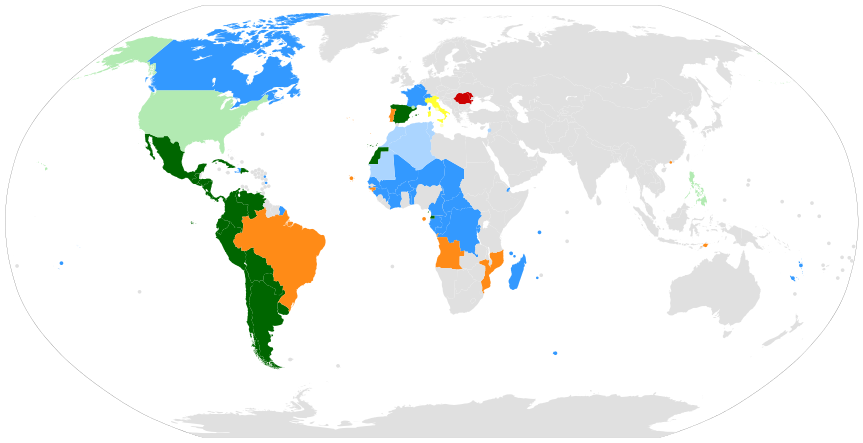
\includegraphics[width=0.9\textwidth]{images/WorldMap.png}
\caption{分布图}
\end{figure}

\section{发展}
\label{sec:org60d44ad}

\begin{enumerate}
\item 演化
\label{sec:orgca7bdeb}

罗曼诸语言中使用者最多的是西班牙语,其后依次是葡萄牙语、法语、意大利语和罗马尼亚语。

在现代的罗曼诸语言中,拉丁语复杂的屈折变化和语法结构已经被大大简化。意大利语、萨丁尼亚语和古典拉丁语最接近。

在罗曼诸语言发展的历史中,最先从拉丁语中分裂出来成为独立语言的是萨丁尼亚語,随之而来的是东部的罗马尼亚语也与拉丁语脱离,成为独立语言。第三个重要过程是意大利语与高卢-伊比利亚语言的分离。这个时候,法国和伊比利亚半岛诸国的语言仍然具有高度的一致性。罗曼语言的第四次重大变化是伊比利亚半岛的语言和法语脱离,逐渐形成非常相似的两种现代语言:西班牙语和葡萄牙语。而通行于西班牙东部的加泰罗尼亚语则被认为是法语和伊比利亚语言的中间产物,因为这种语言融合了法语和西、葡两种语言的很多特征。

\begin{figure}[H]
\centering
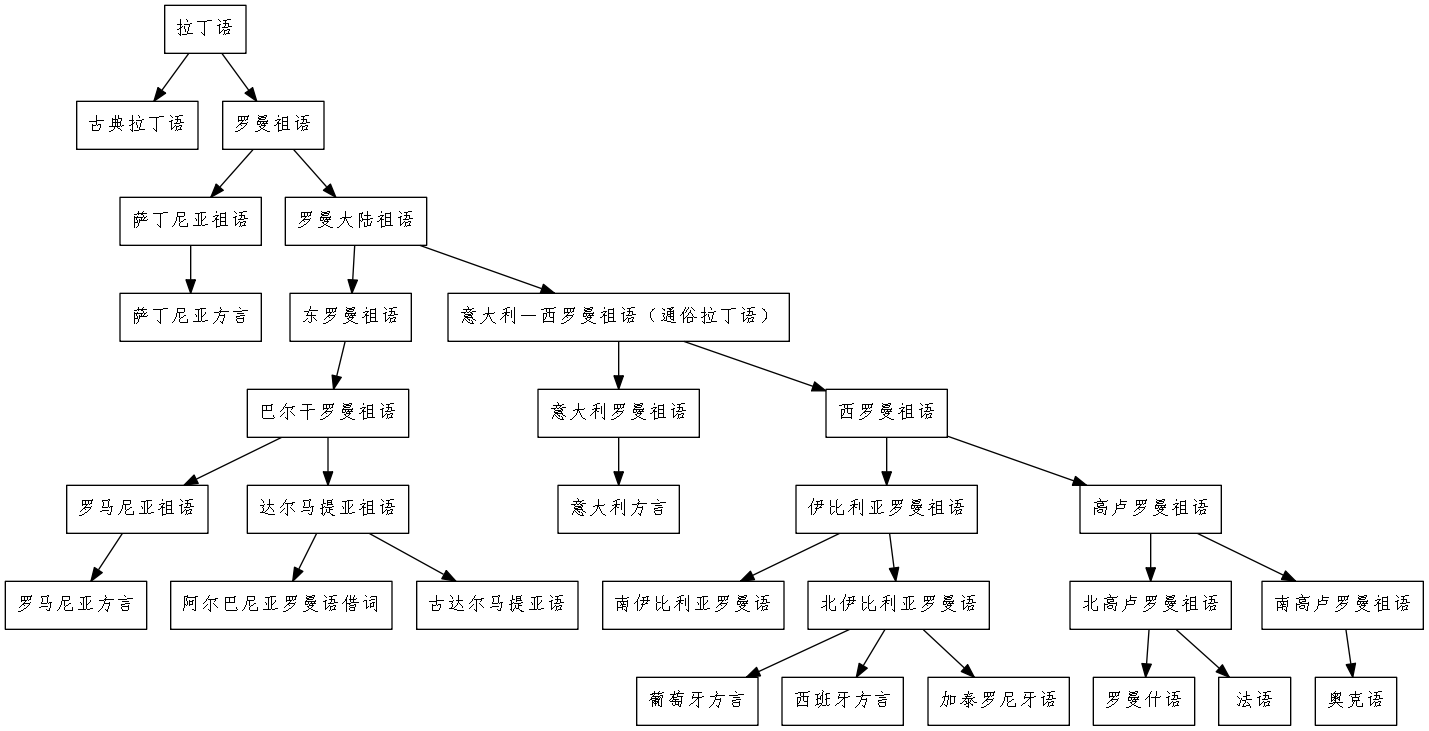
\includegraphics[width=0.9\textwidth]{images/FamilyMap.png}
\caption{演化图}
\end{figure}

\item 分支
\label{sec:org334bd9c}

\begin{itemize}
\item 东罗曼语支
\begin{itemize}
\item 罗马尼亚语 (ron)
\item 伊斯特拉-罗马尼亚语(Romanian, Istro)(ruo)
\item 阿罗马尼亚语、马其顿-罗马尼亚语(Romanian, Macedo)(rup)
\item 梅戈来诺-罗马尼亚语(Romanian, Megleno)(ruq)
\end{itemize}
\item 意大利-西罗曼语支
\begin{itemize}
\item 意大利-达尔马提亚语支
\begin{itemize}
\item 达尔马提亚语(Dalmatian)(dlm)(已灭绝)
\item 伊斯特拉语(Istriot)(ist)
\item 意大利语 (ita)
\item 犹太-意大利语(Judeo-Italian)(itk)
\item 拿坡里语 (nap)
\item 西西里语 (scn)
\item 科西嘉语 Corsican(cos)(一说属于南罗曼语支)
\end{itemize}
\item 西罗曼语支
\begin{itemize}
\item 高卢-意大利语支 Gallo-Italian
\begin{itemize}
\item 艾米利亚-罗马涅语(Emiliano-Romagnolo)(eml)
\item 利古里亚语(Ligurian)(lij)
\item 伦巴底语 (lmo)
\item 皮埃蒙特语 (pms)
\item 威尼斯语 (vec)
\end{itemize}
\item 高卢-罗曼语支 Gallo-Romance
\begin{itemize}
\item 奥依语
\begin{itemize}
\item 法语
\begin{itemize}
\item 古法语 (fro)
\item 盎格鲁-诺曼语 (xno)
\item 法语 (fra)
\item 卡真法语、路易斯安那州法语(Cajun French)(frc)
\item 庇卡底语(Picard)(pcd)
\item 瓦龙语、瓦隆语、华隆语(Wallon)(wln)
\item 查法蒂语、犹太-法语(Zarphatic)(zrp)
\end{itemize}
\end{itemize}
\item 东南奥依语
\begin{itemize}
\item 法兰克-普罗旺斯语(Franco-Provençal)(frp)
\end{itemize}
\item 雷蒂亚-罗曼语(Rhaeto-Romance)
\begin{itemize}
\item 弗留利语 (fur)
\item 拉登语 (lld)
\item 罗曼什语 (roh)
\end{itemize}
\item 奥克-罗曼语(一说属于伊比利亚-罗曼语支下的东伊比利亚语支)
\begin{itemize}
\item 奥克语 (oci)
\item 古普罗旺斯语(Old Provençal)(pro)
\item 苏阿迪特语(Shuadit)(sdt)
\item 加泰罗尼亚语、瓦伦西亚语 (cat)
\end{itemize}
\end{itemize}
\item 伊比利亚-罗曼语支 Ibero-Romance
\begin{itemize}
\item 西伊比利亚语支 West Iberian
\begin{itemize}
\item Asturo-Leonese
\begin{itemize}
\item 阿斯图里亚斯语 (ast)
\item 米兰德斯语(Miranda do Douro)(mwl)
\end{itemize}
\item 卡斯提语 Castilian
\begin{itemize}
\item 埃斯特雷马杜拉语(Extremaduran)(ext)
\item 拉迪诺语、犹太-西班牙语 (lad)
\item 西班牙语 (spa)
\item 洛雷托-乌卡亚利西班牙语、森林西班牙语(Spanish, Loreto-Ucayali,在秘鲁)(spq)
\end{itemize}
\end{itemize}
\end{itemize}
\item 葡萄牙-加利西亚 Portuguese-Galician
\begin{itemize}
\item 法拉语(Fala)(fax)
\item 加利西亚语 (glg)
\item 葡萄牙语 (por)
\end{itemize}
\item 比利牛斯-莫札拉布语支 Pyrenean-Mozarabic
\begin{itemize}
\item 莫札拉布语(Mozarabic)(mxi)
\item 阿拉贡语 (arg)
\end{itemize}
\end{itemize}
\item 南罗曼语支(海岛语支)
\begin{itemize}
\item 古科西嘉语
\item 萨丁尼亚语(Sardinian)(srd)
\begin{itemize}
\item 萨萨里方言(Sardinian, Sassarese)(sdc)
\item 加卢拉方言(Sardinian, Gallurese)(sdn)
\item 劳古多罗方言(Sardinian, Logudorese)(src)
\item 坎皮达诺方言(Sardinian, Campidanese)(sro)
\end{itemize}
\end{itemize}
\end{itemize}
\end{itemize}
\end{enumerate}

\section{比较}
\label{sec:org77fdbb6}

\begin{enumerate}
\item 共同点
\label{sec:org388fd0d}

\begin{itemize}
\item 语法上:
\begin{itemize}
\item 对动作的描述更多的依赖动词自身的变化。语法变化主要依靠动词的词形变化,而非依靠粘着成分。这也是罗曼语言构词法的重要特征。
\item 通常频繁使用两个助动词来构成时态,都是从拉丁语的不定词 esse 和 stare 改变而来的,一个用于描述本质,一个用于描述状态。
\item 动词都要依照人称及数量的不同而进行变位。第三人称通常有语法性的区别,而第一和第二人称则没有。
\item 保留着敬词的痕迹,主要体现在第二人称单数上。
\item 名词都有语法性的区别,但通常只有两种语法性,而拉丁语中名词则有三个语法性。
\item 除罗马尼亚语之外,其他语言已经没有格变化。多以冠词和介词来替代拉丁语词尾复杂的格变化。
\end{itemize}
\item 语音上:
\begin{itemize}
\item 在语音上,通常都将每个词的重音放在倒数第二个音节上(在法语中,重音是放在最后一个音节上的,因为多数法语词汇摈弃了语言词汇的最后一个元音)。
\item 通常都有一些特殊的规定以消除声门塞音、闭塞辅音等对语言整体美感的影响(例如法语中就有“联诵”的规定)。这些特征使得所有的罗曼语言都具有语速快、语调流畅的特点。
\end{itemize}
\item 书写上:
\begin{itemize}
\item 字母 W 和 K 使用得很少,通常只出现在人名和外来语中。
\item 字母 C 和 G 在前元音(如 i、e 等)之前的时候通常读音要软化,在后元音(如 a、o、u)前则要发较硬的软腭音。
\item 一些表示国籍的形容词、表示星期、月份和年份的名词通常首字母不需大写。
\end{itemize}
\end{itemize}

\item 差异点
\label{sec:orgbbdd491}

\begin{itemize}
\item 在一些罗曼语中,名词复数是由名词单数词尾加字母 s 构成的,这是从拉丁语中宾格名词的复数形式演化而来的,以这种方式构成名词复数的罗曼语言包括葡萄牙语、西班牙语、加泰罗尼亚语、普罗旺斯语和法语。也有一些语言的名词复数是由词尾的元音字母变化而构成的,这一特征则是从拉丁语中主格名词的复数形式演化而来。如意大利语和罗马尼亚语等。
\item 一些罗曼语言摈弃了语言词汇的词尾非重读元音。例如欧洲语言的词汇月亮在意大利语中仍是 luna,而在法语中则变成了 lune。仍然保留了词尾元音的语言包括葡萄牙语、西班牙语、意大利语和罗马尼亚语。而法语则摈弃了词尾元音。
\item 罗曼诸语言的比较级构成词也有两种,一种是使用 plus 一词的,一种则是使用 magis 一词的。采用前一种构成方式的语言包括法语(plus)和意大利语(più);而采用后一种构成方式的则包括葡萄牙语(mais)、西班牙语(más)、加泰罗尼亚语(més)等。
\item 在罗曼语言中,“16”这个数字在计数体系中地位非常特殊。除了罗马尼亚语以外,罗曼语言普遍用“1+10”,“2+10”……结构表示 11-15,用“10+7”,“10+8”……结构表示 17-19。而 16 作为两组之间的分界线,在各语言中表达方法不同,其中法语、加泰罗尼亚语、意大利语等用“6+10”表示;而葡萄牙语和西班牙语等则用“10+6”表示。
\item 有些罗曼语言用表达“有”这一含义的助动词来构成复合时态(比如法语中的“愈过去时”等),而有些语言则对动词做出区分,有些动词用“有”来构成,有些则要用“是”来构成。仅使用“有”构成的语言包括加泰罗尼亚语、葡萄牙语、西班牙语和罗马尼亚语等。而混合使用两个助动词的语言则包括法语、意大利语和普罗旺斯语等。在后一类罗曼语言中,用“是”来构成的复合时态的动词通常是常用的不及物动词,这类动词通常描述的是无法确定目标或标明状态的动作。例如“来”、“去”、“变为”等等。而大多数动词还是要利用“有”来构成复合时态。
\end{itemize}
\end{enumerate}

\chapter{辨识}
\label{sec:org46ce1f2}

\begin{itemize}
\item \textbf{一看}
\begin{itemize}
\item c 下面带勾的(ç)一定是法语;n 上面带波浪的(ñ),有特殊标点的(问号 ¿?、叹号 ¡!)一定是西班牙语;双辅音较多的一定是意大利语。
\item 元音上面只有左撇的(闭音符),一定是西班牙语;同时有左撇和右撇(开音符)的,是意大利语;不但有左撇和右撇,还有帽子(长音符)的,一定是法语。
\end{itemize}
\item \textbf{二听}
\begin{itemize}
\item 带小舌颤音的一定是法语;发音有很多 -s 的一定是西班牙语;腔调比较特别的是意大利语。
\end{itemize}
\end{itemize}

\part{语音}
\label{sec:orgd724c47}

\chapter{字母}
\label{sec:org0b3d348}

\section{字母表}
\label{sec:orgf51544e}

\begin{enumerate}
\item Français
\label{sec:orgf338d00}

\begin{longtabu} to 0.9\textwidth {XXX|XXX}
\caption{法语字母表}
\\
\toprule
字母 & 名称 & 读音 & 字母 & 名称 & 读音\\
\midrule
\endfirsthead
\multicolumn{6}{l}{Continued from previous page} \\
\toprule

字母 & 名称 & 读音 & 字母 & 名称 & 读音 \\

\midrule
\endhead
\midrule\multicolumn{6}{r}{Continued on next page} \\
\endfoot
\endlastfoot
A a & a & \textipa{[A]} & N n & enne & \textipa{[En]}\\
B b & bé & \textipa{[be]} & O o & o & \textipa{[o]}\\
C c & cé & \textipa{[se]} & P p & pé & \textipa{[pe]}\\
D d & dé & \textipa{[de]} & Q q & qu & \textipa{[ky]}\\
E e & e & \textipa{[@]} & R r & erre & \textipa{[E:K]}\\
F e & eff & \textipa{[Ef]} & S s & esse & \textipa{[Es]}\\
G g & gé & \textipa{[Ze]} & T t & té & \textipa{[te]}\\
H h & hache & \textipa{[AS]} & U u & u & \textipa{[y]}\\
I i & i & \textipa{[i]} & V v & vé & \textipa{[ve]}\\
J j & ji & \textipa{[Zi]} & W w & double vé & \textipa{[dubl@ve]}\\
K k & ka & \textipa{[kA]} & X x & ixe & \textipa{[iks]}\\
L l & elle & \textipa{[El]} & Y y & i grec & \textipa{[igKEk]}\\
M m & emme & \textipa{[Em]} & Z z & zède & \textipa{[zEd]}\\
\bottomrule
\end{longtabu}

\item Español
\label{sec:org5723ec3}

\begin{longtabu} to 0.9\textwidth {XXX|XXX}
\caption{西班牙语字母表}
\\
\toprule
字母 & 名称 & 读音 & 字母 & 名称 & 读音\\
\midrule
\endfirsthead
\multicolumn{6}{l}{Continued from previous page} \\
\toprule

字母 & 名称 & 读音 & 字母 & 名称 & 读音 \\

\midrule
\endhead
\midrule\multicolumn{6}{r}{Continued on next page} \\
\endfoot
\endlastfoot
A a & a & \textipa{[A]} & N n & ene & \textipa{[ene]}\\
B b & be & \textipa{[be]} & Ñ ñ & eñe & \textipa{[e\textltailn e]}\\
C c & ce & \textipa{[Te]} & O o & o & \textipa{[o]}\\
CH ch & che & \textipa{[tSe]} & P p & pe & \textipa{[pe]}\\
D d & de & \textipa{[de]} & Q q & cu & \textipa{[ku]}\\
E e & e & \textipa{[e]} & R r & ere & \textipa{[eRe]}\\
F e & efe & \textipa{[efe]} & RR rr & erre & \textipa{[ere]}\\
G g & ge & \textipa{[xe]} & S s & ese & \textipa{[ese]}\\
H h & hache & \textipa{[AtSe]} & T t & te & \textipa{[te]}\\
I i & i & \textipa{[i]} & U u & u & \textipa{[u]}\\
J j & jota & \textipa{[xotA]} & V v & uve & \textipa{[uBe]}\\
K k & ca & \textipa{[kA]} & W w & uve doble & \textipa{[uBedoBle]}\\
L l & ele & \textipa{[ele]} & X x & equis & \textipa{[ekis]}\\
LL ll & elle & \textipa{[eJe]} & Y y & i griega & \textipa{[igriegA]}\\
M m & eme & \textipa{[eme]} & Z z & zeta & \textipa{[Teta]}\\
\bottomrule
\end{longtabu}

\begin{itemize}
\item 在西班牙语中,字母 ``K'' 和 ``W'' 平常时一般不用,它们只出现于外来词汇。
\end{itemize}

\item Italiano
\label{sec:org80fe7d2}

\begin{longtabu} to 0.9\textwidth {XXX|XXX}
\caption{意大利语字母表}
\\
\toprule
字母 & 名称 & 读音 & 字母 & 名称 & 读音\\
\midrule
\endfirsthead
\multicolumn{6}{l}{Continued from previous page} \\
\toprule

字母 & 名称 & 读音 & 字母 & 名称 & 读音 \\

\midrule
\endhead
\midrule\multicolumn{6}{r}{Continued on next page} \\
\endfoot
\endlastfoot
A a & a & \textipa{[A]} & N n & enne & \textipa{[enne]}\\
B b & bi & \textipa{[bi]} & O o & o & \textipa{[o]}\\
C c & ci & \textipa{[tSi]} & P p & pi & \textipa{[pi]}\\
D d & di & \textipa{[di]} & Q q & cu & \textipa{[ku]}\\
E e & e & \textipa{[e]} & R r & erre & \textipa{[erre]}\\
F e & effe & \textipa{[effe]} & S s & esse & \textipa{[esse]}\\
G g & gi & \textipa{[dZi]} & T t & ti & \textipa{[ti]}\\
H h & acca & \textipa{[AkkA]} & U u & u & \textipa{[u]}\\
I i & i & \textipa{[i]} & V v & vu & \textipa{[vu]}\\
J j & i lungo & \textipa{[ilungo]} & W w & doppia vu & \textipa{[doppiAvu]}\\
K k & cappa & \textipa{[kAppA]} & X x & ics & \textipa{[iks]}\\
L l & elle & \textipa{[elle]} & Y y & ipsilon & \textipa{[ipsilon]}\\
M m & emme & \textipa{[emme]} & Z z & zeta & \textipa{[tseta]}\\
\bottomrule
\end{longtabu}

\begin{itemize}
\item 在意大利语中,字母 ``J''、``K''、``W''、``X''、``Y'' 只用于外来词汇。
\end{itemize}
\end{enumerate}

\section{音符表}
\label{sec:org506b61e}

\begin{longtabu} to 0.9\textwidth {X|X|X|X}
\caption{音符汇总表}
\\
\toprule
音符名 & 法语适用字母 & 西班牙语适用字母 & 意大利语适用字母\\
\midrule
\endfirsthead
\multicolumn{4}{l}{Continued from previous page} \\
\toprule

音符名 & 法语适用字母 & 西班牙语适用字母 & 意大利语适用字母 \\

\midrule
\endhead
\midrule\multicolumn{4}{r}{Continued on next page} \\
\endfoot
\endlastfoot
闭音符 & é & á, é, í, ó, ú, ý & é, ó\\
开音符 & à, è, ù & - & à, è, ì, ò\\
长音符 & â, ê, î, ô, û & - & -\\
分音符 & ë, ï, ü, ÿ & ï, ü & -\\
软音符 & ç & - & -\\
颚化符 & - & ñ & -\\
\bottomrule
\end{longtabu}

\chapter{发音}
\label{sec:org5f680d5}

\section{发音总表}
\label{sec:org683c2c2}

\begin{longtabu} to 0.9\textwidth {l|X|X|X}
\caption{元音汇总表}
\\
\toprule
音标 & 法语 & 西班牙语 & 意大利语\\
\midrule
\endfirsthead
\multicolumn{4}{l}{Continued from previous page} \\
\toprule

音标 & 法语 & 西班牙语 & 意大利语 \\

\midrule
\endhead
\midrule\multicolumn{4}{r}{Continued on next page} \\
\endfoot
\endlastfoot
\textipa{[A]} & a, à, â & a & a, à\\
\textipa{[E]} & è, ê, ë, ai, aî, ei, -et & e & è\\
\textipa{[e]} & é, -er, -ez, -ed, es- & - & e, é\\
\textipa{[i]} & i, î, ï & i & i, ì, í\\
\textipa{[O]} & o, au[r], & - & ò\\
\textipa{[o]} & o, ô, o[z], au, eau & o & o, ó\\
\textipa{[u]} & ou, où, oû & u & u, ù, ú\\
\textipa{[y]} & u, û & - & -\\
\textipa{[@]} & e & - & -\\
\textipa{[\o]} & eu, œu, eu[zdt] & - & -\\
\textipa{[\oe]} & eu, œu, [cg]ue, œ & - & -\\
\textipa{[\~E]} & in, im, yn, ym, ain, aim, ein, un, um & - & -\\
\textipa{[\~A]} & an, am, en, em & - & -\\
\textipa{[\~O]} & on, om & - & -\\
\bottomrule
\end{longtabu}

\begin{longtabu} to 0.9\textwidth {l|X|X|X}
\caption{辅音汇总表}
\\
\toprule
音标 & 法语 & 西班牙语 & 意大利语\\
\midrule
\endfirsthead
\multicolumn{4}{l}{Continued from previous page} \\
\toprule

音标 & 法语 & 西班牙语 & 意大利语 \\

\midrule
\endhead
\midrule\multicolumn{4}{r}{Continued on next page} \\
\endfoot
\endlastfoot
\textipa{[p]} & p & p & p\\
\textipa{[b]} & b & b-, v- & b\\
\textipa{[B]} & - & -b, -v & -\\
\midrule
\textipa{[t]} & t & t & t\\
\textipa{[d]} & d & d- & d\\
\textipa{[D]} & - & -d- & -\\
\textipa{[T]} & - & -d, z, c-ei & -\\
\midrule
\textipa{[k]} & c-aou, k, ck, qu, -q & c-aou, qu-ei & c-aou, ch-ei\\
\textipa{[g]} & g-aou, gu-eiy & g-aou, gu-ei & g-aou, gh-ei\\
\textipa{[x]} & - & j, g-ei & -\\
\midrule
\textipa{[s]} & s, ss, c-eiy, ç, x & s, x & s\\
\textipa{[z]} & z, zz, -s-, x & - & -s-\\
\midrule
\textipa{[f]} & f, ff, ph & f & f\\
\textipa{[v]} & v & - & v\\
\midrule
\textipa{[S]} & ch & - & sc-ei\\
\textipa{[Z]} & j, g-eiy & - & -\\
\midrule
\textipa{[tS]} & - & ch & c-ei\\
\textipa{[dZ]} & - & - & g-ei\\
\midrule
\textipa{[ts]} & - & - & z\\
\textipa{[dz]} & - & - & z\\
\midrule
\textipa{[m]} & m & m & m\\
\textipa{[n]} & n & n & n\\
\textipa{[\textltailn]} & gn & ñ & gn\\
\textipa{[l]} & l & l & l\\
\textipa{[L]} & - & - & gli\\
\textipa{[J]} & - & ll, y- & -\\
\textipa{[r]} & - & rr & r\\
\textipa{[R]} & - & r & -\\
\textipa{[K]} & r & - & -\\
\midrule
\textipa{[j]} & i-, -il, -ill, y- & i- & i-\\
\textipa{[w]} & ou-, w & u-, w & u-, w\\
\textipa{[4]} & u- & - & -\\
\bottomrule
\end{longtabu}

\section{发音规则}
\label{sec:orgf31aa87}

\begin{enumerate}
\item Français
\label{sec:org0b4dc2d}

\begin{longtabu} to 0.9\textwidth {X|l|X}
\caption{法语元音表}
\\
\toprule
字母组合 & 读音 & 例词\\
\midrule
\endfirsthead
\multicolumn{3}{l}{Continued from previous page} \\
\toprule

字母组合 & 读音 & 例词 \\

\midrule
\endhead
\midrule\multicolumn{3}{r}{Continued on next page} \\
\endfoot
\endlastfoot
a, à, â & \textipa{[A]} & banane, là, fâché\\
e 在 mm 或 nn 前(少数词) &  & femme, solennel\\
\midrule
è, ê, ë & \textipa{[E]} & mère, fête, noël\\
ai, aî, ei &  & lait, maître, reine\\
e 在闭音节中 &  & mer, service, respect\\
e 在两个相同的辅音字母前(m, n 除外) &  & belle, cette, adresse\\
-et 在词末 &  & poulet, filet\\
\midrule
é & \textipa{[e]} & été, léger\\
-er, -ez, -ed 在词尾 &  & loger, visiter, parler, chez, pied\\
es 在单音节词中 &  & les, des, ces\\
ess-, eff-, desc-, dess- 在词首 &  & essai, effet, descendre, dessert\\
\midrule
i, î, ï 及 y & \textipa{[i]} & petit, finir, île, maïs, bicyclette\\
\midrule
u 和 û & \textipa{[y]} & tu, but, flûte, sûr, culture\\
\midrule
ou,où,oû & \textipa{[u]} & loup, où, coût\\
\midrule
ô & \textipa{[o]} & tôt, allô\\
o 在\textipa{[z]}音前 &  & chose, rose\\
o 在词末开音节中 &  & vélo, mot\\
au &  & chaud, cause\\
eau &  & beau, bureau\\
\midrule
o 除发\textipa{[o]}音的情况以外 & \textipa{[O]} & robe, porte, photo\\
au 在 r 前 &  & aurore, aurai\\
\midrule
e 在单音节词中 & \textipa{[@]} & le, te, de, ce\\
e 在词首开音节中 &  & venir, lever, demain\\
e 在“辅辅-e-辅”结构中 &  & entreprise, mercredi, partenaire\\
\midrule
eu, œu 在词末开音节中 & \textipa{[\o]} & peu, deux, vœu, nœud\\
eu 在\textipa{[z]}前 &  & heureuse, vendeuse\\
eu 在\textipa{[d][t][tr]}前 &  & jeudi, émeute, neutre\\
\midrule
eu, œu 除了发\textipa{[\o]}音的情况以外 & \textipa{[\oe]} & fleur, peur, seuil, sœur\\
ue 在 c, g 后 &  & accueil, orgueil\\
œ 在少数单词中 &  & œil\\
\midrule
im, in, ym, yn, aim, ain, ein, um, un(后面不是元音或 m, n) & \textipa{[\~E]} & fin, timbre, syndicat, symbole, faim, pain, plein, lundi, commun\\
\midrule
am, an, em, en(后面不是元音或 m, n) & \textipa{[\~A]} & chambre, champagne, ancre, chanter, emporter, remplir, entrer, content\\
\midrule
om, on(后面不是元音或 m, n) & \textipa{[\~O]} & ombre, tomber, rompre, oncle, salon, chanson\\
\bottomrule
\end{longtabu}

\begin{itemize}
\item 字母组合 um, un,其发音\textipa{[\~\oe]},已有被\textipa{[\~E]}替代的趋势。
\end{itemize}

\begin{longtabu} to 0.9\textwidth {X|l|X}
\caption{法语辅音表}
\\
\toprule
字母组合 & 读音 & 例词\\
\midrule
\endfirsthead
\multicolumn{3}{l}{Continued from previous page} \\
\toprule

字母组合 & 读音 & 例词 \\

\midrule
\endhead
\midrule\multicolumn{3}{r}{Continued on next page} \\
\endfoot
\endlastfoot
p, pp & \textipa{[p]} & pape, impact, palace, parc, Philippe, pratique\\
b, bb & \textipa{[b]} & banque, bicyclette, herbe, abbé, Bible\\
\midrule
t, tt & \textipa{[t]} & tête, table, thé, patte, maître\\
d, dd & \textipa{[d]} & madame, date, déjà, addition, adresse\\
\midrule
k, ck & \textipa{[k]} & kilo, ticket\\
c 在 a, o, u, 辅音字母前或词末 & \textipa{[k]} & casser, coller, cube, clé, lac\\
qu & \textipa{[k]} & tonique, qui, quel\\
q 在词末 & \textipa{[k]} & coq, cinq\\
g 在 a, o, u 及辅音字母前 & \textipa{[g]} & gare, goûter, figure, jungle\\
gu 在 e, i, y 前 & \textipa{[g]} & guetter, guide, Guy\\
\midrule
s, ss & \textipa{[s]} & veste, système,adresse, messe\\
c 在 e, i, y 前 & \textipa{[s]} & cinéma, cycle, scientifique, centre\\
ç & \textipa{[s]} & français, leçon\\
t 在 tion 和 tie 中(前面没有 s) & \textipa{[s]} & attention, nation, démocratie, patience\\
x 在少数词中 & \textipa{[s]} & dix, six\\
z, zz & \textipa{[z]} & gaz, seize, zéro, jazz\\
s 在两个元音字母之间 & \textipa{[z]} & base, visage, paisible\\
x 在个别词中 & \textipa{[z]} & deuxième, sixième\\
\midrule
ch & \textipa{[S]} & Chine, douche\\
j & \textipa{[Z]} & je, jour\\
g 在 e, i, y 前 & \textipa{[Z]} & geste, gilet, gymnastique\\
\midrule
f, ff, ph & \textipa{[f]} & flamme, difficile, chef, philosophie\\
v & \textipa{[v]} & veste, vivre, voir\\
\midrule
l & \textipa{[l]} & loi, facile, allocution, fil, cil\\
m & \textipa{[m]} & ma, pomme, image, mythe\\
n, nn & \textipa{[n]} & minute, année\\
mn 在少数单词中 & \textipa{[n]} & condamner, automne\\
gn & \textipa{[\textltailn]} & signe, campagne, gagner, magnifique, digne\\
r, rr & \textipa{[K]} & rare, mer, gris, bracelet, prune, crèche, Méditerranée\\
\midrule
ou 在元音前 & \textipa{[w]} & jouer, mouette, oui, souhait\\
w 在少数外来词中 & \textipa{[w]} & watt\\
\midrule
i 在元音前 & \textipa{[j]} & lien, ciel, faïence\\
il 在词末且在元音后 & \textipa{[j]} & réveil, travail\\
ill 在元音后 & \textipa{[j]} & bataille, travailler\\
字母 y 在元音前或在词首 & \textipa{[j]} & Lyon, yeux\\
\midrule
u 在元音前 & \textipa{[4]} & nuit lui, fruit, juin\\
\bottomrule
\end{longtabu}

\begin{itemize}
\item 除联诵时,词尾的 d, g, p, s, t, x 和 z 一般不发音。
\end{itemize}

\item Español
\label{sec:orgdbfa337}

\begin{longtabu} to 0.9\textwidth {X|l|X}
\caption{西班牙语元音表}
\\
\toprule
字母组合 & 读音 & 例词\\
\midrule
\endfirsthead
\multicolumn{3}{l}{Continued from previous page} \\
\toprule

字母组合 & 读音 & 例词 \\

\midrule
\endhead
\midrule\multicolumn{3}{r}{Continued on next page} \\
\endfoot
\endlastfoot
a & \textipa{[A]} & ala, amigo\\
e & \textipa{[E]} & eco, esta\\
i & \textipa{[i]} & idea, isla\\
o & \textipa{[o]} & oso, solo\\
u & \textipa{[u]} & uva, luz\\
\midrule
ai, ay & \textipa{[Ai]} & aire, hay\\
ei, ey & \textipa{[Ei]} & seis, peine\\
oi, py & \textipa{[oi]} & oigo, hoy\\
ui, uy & \textipa{[wi]} & ruido, muy\\
au & \textipa{[Au]} & aula, autor\\
eu & \textipa{[Eu]} & neuro, Europa\\
ou & \textipa{[ou]} & bou\\
ia & \textipa{[jA]} & Asia, limpia\\
ie & \textipa{[jE]} & siete, pie\\
io & \textipa{[jo]} & Dios, sucio\\
iu & \textipa{[ju]} & ciudad, viuda\\
ua & \textipa{[wA]} & agua, cuatro\\
ue & \textipa{[wE]} & nuevo, luego\\
uo & \textipa{[wo]} & cuota, antiguo\\
\midrule
iai & \textipa{[jAi]} & cambiáis\\
iei & \textipa{[jEi]} & cambiéis\\
uai, uay & \textipa{[wAi]} & Paraguay\\
uei, uey & \textipa{[wEi]} & buey\\
\bottomrule
\end{longtabu}

\begin{itemize}
\item 西班牙语有五个元音。
\item 以 n, s 或元音字母结尾的单词,重音一般在倒数第二个音节上,不用重音符号。
\item 除了以 n, s 以外的以辅音字母结尾的词,重音位于最后一个音节上,不用重音符号。
\item 上述两项以外的单词,重音都标出:á, é, í, ó, ú。
\end{itemize}

\begin{longtabu} to 0.9\textwidth {X|l|X}
\caption{西班牙语辅音表}
\\
\toprule
字母组合 & 读音 & 例词\\
\midrule
\endfirsthead
\multicolumn{3}{l}{Continued from previous page} \\
\toprule

字母组合 & 读音 & 例词 \\

\midrule
\endhead
\midrule\multicolumn{3}{r}{Continued on next page} \\
\endfoot
\endlastfoot
p & \textipa{[p]} & pa, pe, pi, po, pu, paja, pala, pasta, pata\\
b, v 词首或者位于 m、n 之后时 & \textipa{[b]} & ba, be, bi, bo, bu, bala, boca, voz, vuelo\\
b, v 其他情况 & \textipa{[B]} & -ba, -be, -bi, -bo, -bu, abril, abeja, ava, eve\\
f & \textipa{[f]} & fa, fe, fi,fo, fu, fama\\
\midrule
t & \textipa{[t]} & ta, te, ti, to, tu, tres, talla\\
d 在词首及 n、l 之后 & \textipa{[d]} & da, de, di, do, du, doce, ducha\\
d 位于其他字母之间时 & \textipa{[D]} & -da, -de, -di, -do, -du, verde, lado\\
d 位于词末 & \textipa{[T]} & red, pared\\
\midrule
c 在 a, o, u 前、qu 在 e, i 前 & \textipa{[k]} & ca, que, qui, co, cu, cabo, copa\\
g 在 a, o, u 前、gu 在 e, i 前 & \textipa{[g]} & ga, gue, gui, go, gu, gato, gana\\
g 在 e, i 前 & \textipa{[x]} & ge, gi, gente, gesto\\
j & \textipa{[x]} & ja, je, ji ,jo, ju, jada, jadea\\
\midrule
s、x 位于词首或者辅音前 & \textipa{[s]} & sa, se, si, so, su, sol, seis, extra, sexto\\
x 位于元音前 & \textipa{[ks]} & taxi, exacto\\
z & \textipa{[T]} & za, ze, zi, zo, zu, zumo, zapato\\
c 在 e, i 前 & \textipa{[T]} & ce, ci, cero, ceja\\
\midrule
ch & \textipa{[tS]} & cha, che, chi, cho, chu, chica, chapa\\
\midrule
m & \textipa{[m]} & ma, me, mi, mo, mu, mes, madre\\
n & \textipa{[n]} & na, ne, ni, no, nu, nada, ingenio\\
ñ & \textipa{[\textltailn]} & ña, ñe, ñi, ño, ñu, año, niño\\
l & \textipa{[l]} & la, le, li, lo, lu, ley, labio\\
ll、y 在元音前 & \textipa{[J]} & lla, lle, lli, llo, llu, llave, llanto, yeso\\
y 在元音后或单独出现 & \textipa{[i]} & y, hay\\
r 在词首、rr & \textipa{[r]} & ra, re, ri, ro, ru, corre, Andorra\\
r 不在词首 & \textipa{[R]} & caro, pero\\
\bottomrule
\end{longtabu}

\begin{itemize}
\item gue, gui 发音为\textipa{[gE], [gi]};güe, güi 发音为\textipa{[guE], [gui]}。
\item 在西班牙南部、南美,没有\textipa{[T]}这个音,都发成\textipa{[s]}。
\item -ción 发音为\textipa{[sion]}。
\item w 用来拼写外来词,发音为\textipa{[w]},如 watt, whisky。
\end{itemize}

\item Italiano
\label{sec:org9a80444}

\begin{longtabu} to 0.9\textwidth {X|l|X}
\caption{意大利语元音表}
\\
\toprule
字母组合 & 读音 & 例词\\
\midrule
\endfirsthead
\multicolumn{3}{l}{Continued from previous page} \\
\toprule

字母组合 & 读音 & 例词 \\

\midrule
\endhead
\midrule\multicolumn{3}{r}{Continued on next page} \\
\endfoot
\endlastfoot
à, a & \textipa{[A]} & mamma, papà, vacca, fama, sala\\
è 开口音 & \textipa{[E]} & bène, sètte, bèllo, pèsca, vènto\\
é 闭口音, e & \textipa{[e]} & pésca, vénti, véla, céna, pépe\\
ì, i & \textipa{[i]} & tigre, pini, nidi, lì, sì\\
ò 开口音 & \textipa{[O]} & gònna, mòdo, òtto, nòtte, bòtte\\
ó 闭口音, o & \textipa{[o]} & bótte, óra, scópo, lóro, cóme\\
u & \textipa{[u]} & bue, muto, luna, lupo, duro\\
\midrule
ia & \textipa{[jA]} & piano, piaga\\
ie & \textipa{[jE]} & liève, pièno\\
io & \textipa{[jo]} & òdio, Dio\\
iu & \textipa{[ju]} & piùma, fiume\\
\midrule
ua & \textipa{[wA]} & mutua, uguale\\
ue & \textipa{[wE]} & duèllo, duetto\\
ui & \textipa{[ui]} & suino, guida\\
uo & \textipa{[uo]} & tuòno, duolo\\
\midrule
ai & \textipa{[Ai]} & mai\\
ei & \textipa{[Ei]} & lèi\\
oi & \textipa{[oi]} & pòi\\
\midrule
au & \textipa{[Au]} & paura\\
eu & \textipa{[Eu]} & Euròpa\\
\bottomrule
\end{longtabu}

\begin{itemize}
\item 意大利语有七个元音,其中\textipa{[E]}和\textipa{[O]}只出现在重音节。
\item 只有重读音节上的元音 e、o 才有开口音和闭口音之分,非重读音节(包括单音节词)上的元音 e、o 永远发闭口音。
\item 两个元音连在一起,但其中没有元音 i 和 u 做半元音,就不是二合元音。
\begin{itemize}
\item i 和 u 在另一个元音之前,如:ia, ie, io, iu; ua, ue, uo, ui,称为上升的二合元音,发音时要突出 i 和 u,然后自然地转为 a, e, o, u, i 等音。
\item i 和 u 若在另一个元音之后出现,如:ai, ei, oi, au, eu,称为下降的二合元音,发音时要重读 a, e, o 等元音,随后转发 i 和 u 的音,不要重读。
\end{itemize}
\item 三个元音连在一起同时出现,其中包括元音 i 和 u 的为三合元音。
\item 二合元音、三合元音必须带有 i 或 u。
\end{itemize}

\begin{longtabu} to 0.9\textwidth {X|l|X}
\caption{意大利语辅音表}
\\
\toprule
字母组合 & 读音 & 例词\\
\midrule
\endfirsthead
\multicolumn{3}{l}{Continued from previous page} \\
\toprule

字母组合 & 读音 & 例词 \\

\midrule
\endhead
\midrule\multicolumn{3}{r}{Continued on next page} \\
\endfoot
\endlastfoot
p & \textipa{[p]} & pa, pe, pi, po, pu, pane, pipa, pepe, pupa, lupo, penna, palla\\
b & \textipa{[b]} & ba, be, bi, bo, bu, basta, bene, bella, buono, bimbo, bomba\\
\midrule
t & \textipa{[t]} & ta, te, ti, to, tu, letto, lotta, tanto, tutto, notte, alto, molto\\
d & \textipa{[d]} & da, de, di, do, du, dente, modo, mondo, debole, dubbio, moda\\
\midrule
c 在 a, o, u 前, 或 ch 在 e, i 之前 & \textipa{[k]} & ca, che, chi, co, cu, come, casa, cosa, bocca, amico, pacco, anche, capo\\
g 在 a, o, u 前, 或 gh 在 e, i 之前 & \textipa{[g]} & ga, ghe, ghi, go, gu, gamba, gonna, gola, gusto, gatto, gomma\\
\midrule
s & \textipa{[s]} & sa, se, si, so, su, sala, sole, sale, solo, testa, sedia\\
s 在两个元音之间, 或在浊辅音 b,d,g,l,m,n,v 之前 & \textipa{[z]} & peso, naso, smalto, sviluppo\\
\midrule
c 在 e, i 之前 & \textipa{[tS]} & ce, ci, cima, cinema, cemento, cibo, dolce, calcio\\
g 在 e, i 之前 & \textipa{[dZ]} & ge, gi, gita, gesto, oggi, giacca, giallo, gente, gentile\\
\midrule
f & \textipa{[f]} & fa, fe, fi, fo, fu, fame, fare, fumo, folla, fede, festa, frutta\\
v & \textipa{[v]} & va, ve, vi, vo, vu, vaso, vino, visa, voto, vuoto, vecchio, tavolo\\
\midrule
z & \textipa{[ts]} & za, ze, zi, zo, zu, zappa, zoppo, zucca, zitto, pezzo, pazzo, zio\\
z & \textipa{[dz]} & za, ze, zi, zo, zu, zona, zelo, zoo, mezzo, zaino, bronzo\\
\midrule
m & \textipa{[m]} & ma, me, mi, mo, mu, mamma, amo, ama, mimo, mela, miele\\
n & \textipa{[n]} & na, ne, ni, no, nu, nonno, nome, meno, uno, notte, mano, ninna\\
gn & \textipa{[\textltailn]} & gna, gne, gni, gno, gnu, ogni, ragno, sogna, legno, signore, bagno, montagna\\
l & \textipa{[l]} & la, le, li, lo, lu, lana, male, lama, lino, luna, mille, mila\\
r & \textipa{[r]} & ra, re, ri, ro, ru\\
\midrule
sc 在 e, i 之前 & \textipa{[S]} & scia, sce, sci, scio, sciu, scimmia, sciopero, scena, pesce, ascia\\
sc 在 a, o, u, he, hi 之前 & \textipa{[sk]} & sca, sco, scu, scuola, scherzo, schiuma, scopa, pesca\\
\midrule
gl 在 i 之前,或 gli 在 a, e, o, u 之前 & \textipa{[L]} & glia, glie, gli, glio, gliu, maglia, moglie, luglio, meglio\\
gl 在 a, e, o, u 之前 & \textipa{[gl]} & gloria, gleba, glucosio\\
\bottomrule
\end{longtabu}

\begin{itemize}
\item 意大利语中 h 在任何位置都是不发音的,但是 h 起到指示发音的作用。
\item 双辅音要适当延长其发音的阻塞时间。辅音都能延长,除了\textipa{[z]}。
\end{itemize}
\end{enumerate}

\part{语法}
\label{sec:org268c827}

\chapter{名词}
\label{sec:org40dd478}

\section{名词}
\label{sec:org9a5d810}

名词有性(阳性、阴性)、数(单数、复数)的变化,基本上不再有格的变化。

\begin{enumerate}
\item Français
\label{sec:org97a965e}

\item Español
\label{sec:org841dbc1}

\item Italiano
\label{sec:orgb6345cf}

\begin{longtabu} to 0.9\textwidth {l|X|X}
\caption{意大利语名词单复数表}
\\
\toprule
 & 单数 & 复数\\
\midrule
\endfirsthead
\multicolumn{3}{l}{Continued from previous page} \\
\toprule

 & 单数 & 复数 \\

\midrule
\endhead
\midrule\multicolumn{3}{r}{Continued on next page} \\
\endfoot
\endlastfoot
阳性 & -o & -i\\
 & -a & -i\\
 & -e & -i\\
\midrule
阴性 & -a & -e\\
 & -e & -i\\
\bottomrule
\end{longtabu}

\begin{itemize}
\item 以 a 或 e 结尾的,可能是阳性名词,也可能是阴性名词,要从冠词来区分。
\item 以 ca/ga 结尾的阴性名词,由于发音关系,变为 che/ghe,如 amica-amiche。
\item 以 co/go 结尾的阳性名词,由于发音关系,变为 chi/ghi,如 lago-laghi;但也有改变发音,直接变成 ci/gi,如 amico-amici。
\item 复数不变化的词
\begin{itemize}
\item 重音在末尾音节的,如 città,università,caffè;
\item 单音节词,如 re,tè,gru,pro;
\item 单数是 i 结尾的,如 analisi,crisi,tesi;
\item 辅音结尾的,如 lapis,film,sport,gas。
\end{itemize}
\item 人体器官的名词,复数变化大部分不规则
\begin{center}
\begin{tabular}{lll}
意思 & 单数 & 复数\\
\hline
脑 & il cervello & le cervella\\
眼睛 & l'occhio & gli occhi\\
睫毛 & il ciglio & le ciglia\\
眉毛 & il sopraciglio & le sopraciglia\\
耳朵 & l'orecchio & le orecchie / gli orecchi\\
鼻 & il naso & i nasi\\
嘴 & la bocca & le bocche\\
嘴唇 & il labbro & le labbra\\
胳膊 & il braccio & le braccia\\
腿 & la gamba & le gambe\\
膝盖 & il ginocchio & i ginocchi / le ginocchia\\
手 & la mano & le mani\\
手指、脚趾 & il dito & i diti / le dita\\
指甲 & l'unghia & le unghie\\
骨 & l'osso / le ossa & gli ossi\\
皮 & il cuoio & le cuoia\\
肌肉 & il muscolo & i muscoli\\
脚 & il piede & i piedi\\
\end{tabular}
\end{center}
\end{itemize}
\end{enumerate}

\chapter{冠词}
\label{sec:orga4a8d07}

\section{冠词}
\label{sec:orgebd0ba9}

冠词有性(阳性、阴性)、数(单数、复数)的变化,要和其限定的名词做性数配合。

\begin{enumerate}
\item Français
\label{sec:org6140520}

\begin{longtabu} to 0.9\textwidth {l|X|X|X}
\caption{法语定冠词表}
\\
\toprule
 & 规则 & 单数 & 复数\\
\midrule
\endfirsthead
\multicolumn{4}{l}{Continued from previous page} \\
\toprule

 & 规则 & 单数 & 复数 \\

\midrule
\endhead
\midrule\multicolumn{4}{r}{Continued on next page} \\
\endfoot
\endlastfoot
阳性 & 元音前、哑音前 & l' & les\\
 & 辅音前、嘘音前 & le & \\
\midrule
阴性 & 元音前、哑音前 & l' & les\\
 & 辅音前、嘘音前 & la & \\
\bottomrule
\end{longtabu}

\item Español
\label{sec:org7ae05e0}

\begin{longtabu} to 0.9\textwidth {l|X|X|X}
\caption{西班牙定语冠词表}
\\
\toprule
 & 规则 & 单数 & 复数\\
\midrule
\endfirsthead
\multicolumn{4}{l}{Continued from previous page} \\
\toprule

 & 规则 & 单数 & 复数 \\

\midrule
\endhead
\midrule\multicolumn{4}{r}{Continued on next page} \\
\endfoot
\endlastfoot
阳性 &  & el & los\\
\midrule
阴性 &  & la & las\\
\bottomrule
\end{longtabu}

\item Italiano
\label{sec:orgbb7c102}

\begin{longtabu} to 0.9\textwidth {l|X|X|X}
\caption{意大利语定冠词表}
\\
\toprule
 & 规则 & 单数 & 复数\\
\midrule
\endfirsthead
\multicolumn{4}{l}{Continued from previous page} \\
\toprule

 & 规则 & 单数 & 复数 \\

\midrule
\endhead
\midrule\multicolumn{4}{r}{Continued on next page} \\
\endfoot
\endlastfoot
阳性 & 元音前 & l' & gl'(i 前) / gli(其他元音前)\\
 & s+辅音, z, x, y, ps, gn 前 & lo & gli\\
 & 其他辅音前 & il & i\\
\midrule
阴性 & 元音前 & l' & le(在 e 前可省音 l')\\
 & 辅音前 & la & le\\
\bottomrule
\end{longtabu}

\begin{longtabu} to 0.9\textwidth {l|X|X|X}
\caption{意大利语不定冠词表}
\\
\toprule
 & 规则 & 单数 & 复数\\
\midrule
\endfirsthead
\multicolumn{4}{l}{Continued from previous page} \\
\toprule

 & 规则 & 单数 & 复数 \\

\midrule
\endhead
\midrule\multicolumn{4}{r}{Continued on next page} \\
\endfoot
\endlastfoot
阳性 & 元音前 & un & degli\\
 & s+辅音, z, x, y, ps, gn 前 & uno & degli\\
 & 其他辅音前 & un & dei\\
\midrule
阴性 & 元音前 & un' & delle\\
 & 辅音前 & una & delle\\
\bottomrule
\end{longtabu}

\begin{longtabu} to 0.9\textwidth {l|X|X|X|X|X|X}
\caption{意大利语缩合冠词表}
\\
\toprule
介词 & il & lo & la & i & gli & le\\
\midrule
\endfirsthead
\multicolumn{7}{l}{Continued from previous page} \\
\toprule

介词 & il & lo & la & i & gli & le \\

\midrule
\endhead
\midrule\multicolumn{7}{r}{Continued on next page} \\
\endfoot
\endlastfoot
a & al & allo & alla & ai & agli & alle\\
di & del & dello & della & dei & degli & delle\\
da & dal & dallo & dalla & dai & dagli & dalle\\
in & nel & nello & nella & nei & negli & nelle\\
su & sul & sullo & sulla & sui & sugli & sulle\\
con & col & - & - & coi & - & -\\
per & pel & - & - & pei & - & -\\
\bottomrule
\end{longtabu}

\begin{itemize}
\item con、per 的缩合形式不常用,通常还是用 con il、con i、pei il、pei i。
\end{itemize}
\end{enumerate}

\chapter{代词}
\label{sec:org73c17d1}

\section{代词}
\label{sec:org55a1d65}

代词有性(阳性、阴性)、数(单数、复数)的变化。

\begin{enumerate}
\item Français
\label{sec:org87e7de1}

\item Español
\label{sec:orgbfd0f1a}

\item Italiano
\label{sec:org1a7800b}

\begin{longtabu} to 0.9\textwidth {l|X|X|X|X|X|X}
\caption{意大利语人称代词表}
\\
\toprule
 & 人称 & 主格 & 直接补语(重读) & 直接补语(非重读) & 间接补语(重读) & 间接补语(非重读)\\
\midrule
\endfirsthead
\multicolumn{7}{l}{Continued from previous page} \\
\toprule

 & 人称 & 主格 & 直接补语(重读) & 直接补语(非重读) & 间接补语(重读) & 间接补语(非重读) \\

\midrule
\endhead
\midrule\multicolumn{7}{r}{Continued on next page} \\
\endfoot
\endlastfoot
单数 & 我 & io & me & mi & a me & mi\\
 & 你 & tu & te & ti & a te & ti\\
 & 他 & lui & lui/sé & lo/si & a lui/a sé & gli/si\\
 & 她 & lei & lei/sé & la/si & a lei/a sé & le/si\\
\midrule
复数 & 我们 & noi & noi & ci & a noi & ci\\
 & 你们 & voi & voi & vi & a voi & vi\\
 & 他们 & loro & loro/sé & li/si & a loro/a sé & loro/si\\
 & 她们 & loro & loro/sé & le/si & a loro/a sé & loro/si\\
\bottomrule
\end{longtabu}

\begin{itemize}
\item 大写的第三人称阴性单数 Lei 和复数 Loro,可以分别表示尊称“您”和“您们”。口语中,常常用 voi 代替 Loro。
\item 直接补语的重读与非重读对比:La zia chiama voi.(阿姨叫的是你们。)/ La zia vi chiama.(阿姨叫你们。)
\item 间接补语的重读与非重读对比:La zia dà un libro a me.(阿姨把一本书给我。)/ La zia mi dà un libro.(阿姨给我一本书。)
\item lo/la/li/le/ne 分别代词作为直接补语的阳性单数、阴性单数、阳性复数、阴性复数名词,表示全部。ne 表示部分或者一点儿也没有。
Leggi tutti questi libri? - Sì, li leggo. / No, ne leggo solo alcuni. / No, non ne leggo affatto.(这些书你都读吗?是,我都读。/ 不,我只读一些。/ 不,我一本也不读。)
\item 一般情况下,直接补语代词位于变位动词的前面。如果直接补语代词与动词不定式一起使用,应与去掉 e 的动词原形连写,或者置于变位动词前。
\begin{itemize}
\item Lo conosco.(我认识他。)
\item La vogliamo visitare. / Vogliamo visitarla.(我们想要参观它。)
\end{itemize}
\item 间接补语代词代替由前置词 a 引出的间接宾语。通常位于变位动词前。
\begin{itemize}
\item Parlo ai miei amici. → Gli parlo.(我和我的朋友谈话。→ 我和他们谈话。)
\end{itemize}
\item lo/la/li/le 用在变了位的动词 avere 前时,它们的前面要加上 ce,此处 ce 没有实际含义。
Avete tutti i libri necessari? Sì, ce li abbiamo.(你们有所有必需的书籍吗?是的,我们有。)
\item 如果同时有间接补语和直接补语,放在动词后时,先间接后直接。
\begin{itemize}
\item Date a me il libro. → Datemelo.(你们把书给我。→ 你们把它给我。)
\end{itemize}
\item 当间接补语和直接补语连用时,需要写成组合形式:
\begin{itemize}
\item Glieli puoi dare tu?(你能把它们给他吗?)
\end{itemize}
\begin{center}
\begin{tabular}{llllll}
 & lo & la & li & le & ne\\
\hline
mi & me lo & me la & me li & me le & me ne\\
ti & te lo & te la & te li & te le & te ne\\
ci & ce lo & ce la & ce li & ce le & ce ne\\
vi & ve lo & ve la & ve li & ve le & ve ne\\
gli & glielo & gliela & glieli & gliele & gliene\\
\end{tabular}
\end{center}
\end{itemize}

\begin{longtabu} to 0.9\textwidth {l|X|X|X|X}
\caption{意大利语物主代词表}
\\
\toprule
人称 & 阳性单数 & 阳性复数 & 阴性单数 & 阴性复数\\
\midrule
\endfirsthead
\multicolumn{5}{l}{Continued from previous page} \\
\toprule

人称 & 阳性单数 & 阳性复数 & 阴性单数 & 阴性复数 \\

\midrule
\endhead
\midrule\multicolumn{5}{r}{Continued on next page} \\
\endfoot
\endlastfoot
单数第一人称 & mio & miei & mia & mie\\
单数第二人称 & tuo & tuoi & tua & tue\\
单数第三人称 & suo & suoi & sua & sue\\
复数第一人称 & nostro & nostri & nostra & nostre\\
复数第二人称 & vostro & vostri & vostra & vostre\\
复数第三人称 & loro & loro & loro & loro\\
\bottomrule
\end{longtabu}

\begin{itemize}
\item 即在物主形容词前加上相应的定冠词。La sua stanza e più nuova della mia.(他的房间比我的新。)
\end{itemize}

\begin{longtabu} to 0.9\textwidth {l|X|X|X|X}
\caption{意大利语指示代词表}
\\
\toprule
指代 & 阳性单数 & 阳性复数 & 阴性单数 & 阴性复数\\
\midrule
\endfirsthead
\multicolumn{5}{l}{Continued from previous page} \\
\toprule

指代 & 阳性单数 & 阳性复数 & 阴性单数 & 阴性复数 \\

\midrule
\endhead
\midrule\multicolumn{5}{r}{Continued on next page} \\
\endfoot
\endlastfoot
这 & questo & questi & questa & queste\\
那 & codesto & codesti & codesta & codeste\\
那 & quello & quelli & quella & quelle\\
\bottomrule
\end{longtabu}

\begin{longtabu} to 0.9\textwidth {l|X}
\caption{意大利语疑问代词表}
\\
\toprule
 & 变化\\
\midrule
\endfirsthead
\multicolumn{2}{l}{Continued from previous page} \\
\toprule

 & 变化 \\

\midrule
\endhead
\midrule\multicolumn{2}{r}{Continued on next page} \\
\endfoot
\endlastfoot
che 什么 & 不变\\
chi 谁 & 不变\\
quale 哪个 & 数 quale/quali\\
quanto 多少 & 性数 quanto/quanta/quanti/quante\\
\bottomrule
\end{longtabu}

\begin{longtabu} to 0.9\textwidth {l|X|X}
\caption{意大利语关系代词表}
\\
\toprule
 & 变化 & 例句\\
\midrule
\endfirsthead
\multicolumn{3}{l}{Continued from previous page} \\
\toprule

 & 变化 & 例句 \\

\midrule
\endhead
\midrule\multicolumn{3}{r}{Continued on next page} \\
\endfoot
\endlastfoot
che 主语/直接补语 & 不变 & Dammi il libro che è sul tavolo.(把在桌上的书给我。)\\
cui 其他补语 & 不变 & L'uomo, cui mi rivolgo, è gentil.(我求教的人很热情。)\\
chi 单数主语/补语 & 不变 & Chi non ha testa abbia gambe.(没脑子的人就多动腿。)\\
quale 主语/补语 & 性数 il quale/la quele/i quali/le quali & Il treno, col quale sono arrivato, era in ritardo.(我来时乘的火车晚点了。)\\
dove/donde 地点 & 不变 & La città dove abitiamo è molto grande.(我们居住的城市非常大。)\\
\bottomrule
\end{longtabu}
\end{enumerate}

\chapter{形容词}
\label{sec:org315286f}

\section{形容词}
\label{sec:org8ebca4d}

形容词有性(阳性、阴性)、数(单数、复数)的变化,要和其限定的名词做性数配合。

\begin{enumerate}
\item Français
\label{sec:org8df19b3}

\item Español
\label{sec:orgc421bbe}

\item Italiano
\label{sec:org61b13e8}

\begin{longtabu} to 0.9\textwidth {l|X|X|X|X|X}
\caption{意大利语形容词单复数表}
\\
\toprule
形容词原形词尾 & 被修饰的名词 & 单数 & 例子 & 复数 & 例子\\
\midrule
\endfirsthead
\multicolumn{6}{l}{Continued from previous page} \\
\toprule

形容词原形词尾 & 被修饰的名词 & 单数 & 例子 & 复数 & 例子 \\

\midrule
\endhead
\midrule\multicolumn{6}{r}{Continued on next page} \\
\endfoot
\endlastfoot
-o & 阳性名词 & -o & il ragazzo alto & -i & i ragazzi alti\\
 & 阴性名词 & -a & la ragazza alta & -e & le ragazze alte\\
\midrule
-e & 不分阴阳性 & -e & il ragazzo volece & -i & i ragazzi voleci\\
 &  &  & la ragazza volece &  & le ragazze voleci\\
\bottomrule
\end{longtabu}

\begin{itemize}
\item 以 co 结尾的形容词,如果重音在倒数第二音节,变为 chi,如 bianco-bianchi。但有例外,amico-amici,nemico-nemici。如果重音在倒数第三音节,直接变为 ci,如 unico-unici。但也有例外,carico-carichi。
\item 以 go 结尾的形容词,都变为 ghi,如 largo-larghi,lungo-longhi。
\item 以 ca/ga 结尾的,变为 che/ghe,如 unica-uniche,amica-amiche。
\end{itemize}

\begin{longtabu} to 0.9\textwidth {l|X|X}
\caption{意大利语形容词等级表}
\\
\toprule
级别 & 表达 & 例子\\
\midrule
\endfirsthead
\multicolumn{3}{l}{Continued from previous page} \\
\toprule

级别 & 表达 & 例子 \\

\midrule
\endhead
\midrule\multicolumn{3}{r}{Continued on next page} \\
\endfoot
\endlastfoot
同级 & così\ldots{}come,tanto\ldots{}quanto & Mario è così alto come Luigi.\\
较高级 & più\ldots{}di,più\ldots{}che & Mario è più alto di Luigi.\\
较低级 & meno\ldots{}di,meno\ldots{}che & Mario è meno alto di Luigi.\\
相对最高级 & 冠词+più & Mario è l'uomo più alto della classe.\\
相对最低级 & 冠词+meno & Mario è l'uomo meno alto della classe.\\
绝对最高级 & 形容词阳性复数+ssimo & Mario è altissimo.\\
\bottomrule
\end{longtabu}

\begin{itemize}
\item 不同的人、物见之间比较时,通常用 di;同一个人、物的不同特性比较通常用 che。
\item 不规则形容词
\begin{center}
\begin{tabular}{lll}
原级 & 比较级 & 最高级\\
\hline
buono(好的) & migliore & ottimo\\
cattivo(坏的) & peggiore & pessimo\\
grande(大的) & maggiore & massiomo\\
piccolo(小的) & minore & minimo\\
alto(高的) & superiore & supremo, sommo\\
basso(低的) & inferiore & infimo\\
\end{tabular}
\end{center}
\end{itemize}

\begin{longtabu} to 0.9\textwidth {l|X|X|X|X}
\caption{意大利语物主形容词表}
\\
\toprule
人称 & 阳性单数 & 阳性复数 & 阴性单数 & 阴性复数\\
\midrule
\endfirsthead
\multicolumn{5}{l}{Continued from previous page} \\
\toprule

人称 & 阳性单数 & 阳性复数 & 阴性单数 & 阴性复数 \\

\midrule
\endhead
\midrule\multicolumn{5}{r}{Continued on next page} \\
\endfoot
\endlastfoot
单数第一人称 & mio & miei & mia & mie\\
单数第二人称 & tuo & tuoi & tua & tue\\
单数第三人称 & suo & suoi & sua & sue\\
复数第一人称 & nostro & nostri & nostra & nostre\\
复数第二人称 & vostro & vostri & vostra & vostre\\
复数第三人称 & loro & loro & loro & loro\\
\bottomrule
\end{longtabu}

\begin{itemize}
\item 物主形容词需要和被限定的名词的性数配合,还要与定冠词一致。如,il mio libro,la mia casa。
\item 在亲属关系的名词单数前通常省略定冠词,复数前不能省略。如,mio fratello,tua sorella,i miei fratelli,le tue sorelle。但有形容词时,还要保留定冠词。如,il mio giovane fratello,la tua cara sorella。此外,loro 前的定冠词不省略,如 la loro zia。
\end{itemize}

\begin{longtabu} to 0.9\textwidth {l|X|X|X|X}
\caption{意大利语指示形容词表}
\\
\toprule
指代 & 阳性单数 & 阳性复数 & 阴性单数 & 阴性复数\\
\midrule
\endfirsthead
\multicolumn{5}{l}{Continued from previous page} \\
\toprule

指代 & 阳性单数 & 阳性复数 & 阴性单数 & 阴性复数 \\

\midrule
\endhead
\midrule\multicolumn{5}{r}{Continued on next page} \\
\endfoot
\endlastfoot
这 & questo & questi & questa & queste\\
那 & codesto & codesti & codesta & codeste\\
那 & quello & quelli & quella & quelle\\
\bottomrule
\end{longtabu}

\begin{itemize}
\item quello 变化:在辅音开头的名词前要断音(quel),在元音开头的名词前要省音(quell'),在 s/z/gn 前不变(quello)。
\end{itemize}

\begin{longtabu} to 0.9\textwidth {l|X}
\caption{意大利语疑问形容词表}
\\
\toprule
 & 变化\\
\midrule
\endfirsthead
\multicolumn{2}{l}{Continued from previous page} \\
\toprule

 & 变化 \\

\midrule
\endhead
\midrule\multicolumn{2}{r}{Continued on next page} \\
\endfoot
\endlastfoot
che(什么) & 不变\\
quale(哪个) & 数 quale/quali\\
quanto(多少) & 性数 quanto/quanta/quanti/quante\\
\bottomrule
\end{longtabu}
\end{enumerate}

\chapter{数词}
\label{sec:org293ddd4}

\section{数词}
\label{sec:org3a1c175}

数词分基数词和序数词。基数词“1”需要和计数的名词的性一致。序数词要与被计数名词保持性数一致。

\begin{enumerate}
\item Français
\label{sec:org9f97140}

\item Español
\label{sec:orgb7aaaff}

\item Italiano
\label{sec:org0077e0b}

\begin{longtabu} to 0.9\textwidth {l|X|l|X}
\caption{意大利语数词表}
\\
\toprule
数字 & 拼写 & 数字 & 拼写\\
\midrule
\endfirsthead
\multicolumn{4}{l}{Continued from previous page} \\
\toprule

数字 & 拼写 & 数字 & 拼写 \\

\midrule
\endhead
\midrule\multicolumn{4}{r}{Continued on next page} \\
\endfoot
\endlastfoot
1 & uno & 1° & primo\\
2 & due & 2° & scondo\\
3 & tre & 3° & terzo\\
4 & quattro & 4° & quarto\\
5 & cinque & 5° & quinto\\
6 & six & 6° & sesto\\
7 & sette & 7° & settimo\\
8 & otto & 8° & ottavo\\
9 & nove & 9° & nono\\
10 & dieci & 10° & decimo\\
11 & undici & 11° & undicesimo/undecimo\\
12 & dodici & 12° & dodicesimo/duodecimo\\
13 & tredici & 13° & tredicesimo/decimoterzo\\
14 & quattordici & 14° & quattordicesimo/decimoquarto\\
15 & quindici & 15° & quindicesimo/decimoquinto\\
16 & sedici & 16° & sedicesimo/decimosesto\\
17 & diciassette & 17° & diciassettesimo/decimosettimo\\
18 & diciotto & 18° & diciottesimo/decimoottavo\\
19 & diciannove & 19° & diciannovesimo/decimonono\\
20 & venti & 20° & ventesimo\\
21 & ventuno & 21° & ventunesimo/ventesimoprimo\\
22 & ventidue & 22° & ventiduesimo/ventesimosecondo\\
23 & ventitré & 23° & ventitreesimo/ventesimoterzo\\
24 & ventiquattro & 24° & ventiquattresimo/ventesimoquarto\\
25 & venticinque & 25° & venticinquesimo/ventesimoquinto\\
26 & ventisci & 26° & ventiscesimo/ventesimosesto\\
27 & ventisette & 27° & ventisettesimo/ventesimosettimo\\
28 & ventotto & 28° & ventottesimo/ventesimoottavo\\
29 & ventinove & 29° & ventinovesimo/ventesimonono\\
30 & trenta & 30° & trentesimo\\
40 & quaranta & 40° & quarantesimo\\
50 & cinquanta & 50° & cinquantesimo\\
60 & sessanta & 60° & sessantesimo\\
70 & settanta & 70° & settantesimo\\
80 & ottanta & 80° & ottantesimo\\
90 & novanta & 90° & novantesimo\\
100 & cento & 100° & centesimo\\
101 & centouno/centuno & 101° & centesimoprimo\\
111 & centoundici & 111° & centesimoundicesimo/centesimoundecimo\\
120 & centoventi & 120° & centesimoventesimo\\
200 & duecento & 200° & duecentesimo\\
1.000 & mille & 1.000° & millesimo\\
1.001 & milleuno/mille e uno & 1.001° & millesimoprimo\\
1.150 & millecentocinquanta & 1.150° & millesimocentesimocinquantesimo\\
2.000 & duemila & 2.000° & duemillesimo\\
100.000 & centomila & 100.000° & centomillesimo\\
200.000 & duecentomila & 200.000° & duecentomillesimo\\
\bottomrule
\end{longtabu}

\begin{itemize}
\item uno/una 有性的变化,如:uno libro,una sedia。而且“几十一”后面有名词时,需要断音,如:ventun libri,trentun sedie。
\item mille 需变成复数 mila,且连写。如:2.000:duemila,10.000:diecimila。
\item 更大的数字是名词,有数的变化。如 1.000.000:un milione,2.000.000:due milioni,1.000.000.000:un miliardo,2.000.000.000:due miliardi。并且后面不能直接跟名词,需要 di:due milioni di dollari。
\item 表达几点钟时,视作复数。Sono le sette.(七点。)
\item 小数读法:0,07(zero virgola zero sette)。其小数点为``,'',千分位为``.'',和中文相反。
\item 序数词要与被计数名词保持性数一致。如:il primo giorno,la prima sera,i primi passi,le prime rose。
\item 分数读法:分子用基数词,分母用序数词,如:1/3 un terzo,2/3 due terzi,5/8 cinque ottavi。1/2 用 un mezzo。
\item 四则运算:
\begin{itemize}
\item 4+5=9: quattro più cinque eguale nove
\item 7-5=2: sette meno cinque eguale due
\item 25x1=25: venticinque moltiplicato per uno eguale venticinque
\item 85:4=21\ldots{}1: ottantacinque diviso quattro eguale ventuno con il resto di uno
\end{itemize}
\end{itemize}
\end{enumerate}

\chapter{动词}
\label{sec:org7067c85}

\section{动词}
\label{sec:org282a285}

动词有时(现在时、将来时、过去时)、式(直陈式、命令式、虚拟式、条件式)、态(主动态、被动态)、分词(现在分词、过去分词)等各种变化。

\begin{enumerate}
\item Français
\label{sec:orgc45fcc5}

\item Español
\label{sec:org92e8e03}

\item Italiano
\label{sec:org4fd979e}

意大利语动词的时式总览如下:
\begin{figure}[H]
\centering
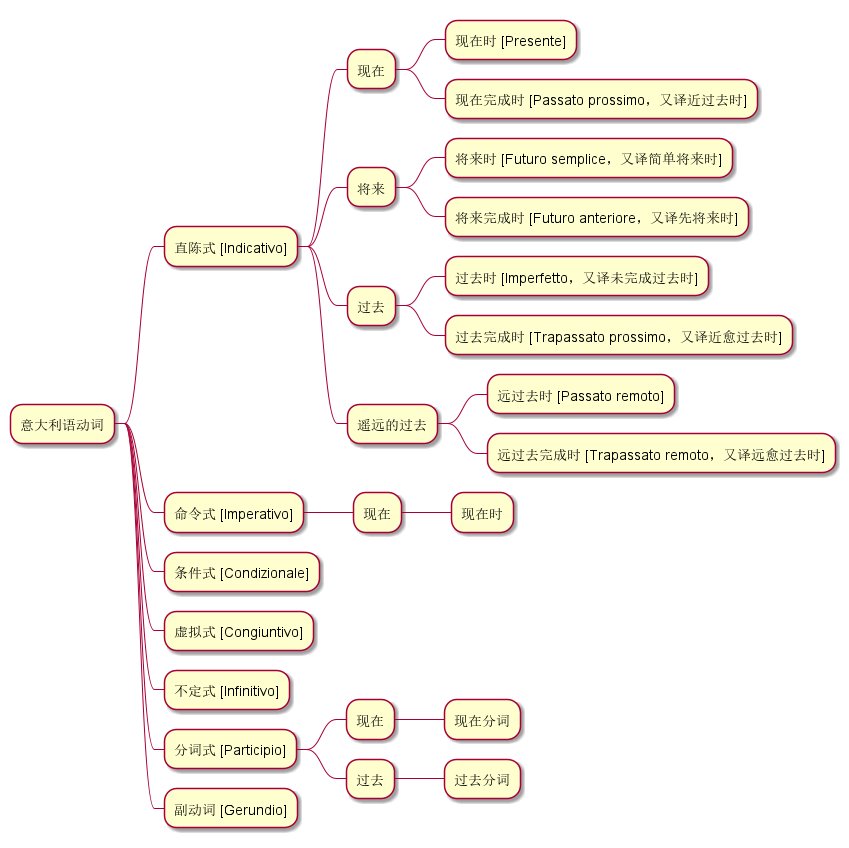
\includegraphics[width=0.9\textwidth]{images/italian-verb.png}
\caption{意大利语动词时式图}
\end{figure}

\begin{longtabu} to 0.9\textwidth {l|X|X|X|X|X|X}
\caption{\label{意大利语直陈式现在时变位表}意大利语直陈式现在时变位表}
\\
\toprule
 & io & tu & lui/lei & noi & voi & loro\\
\midrule
\endfirsthead
\multicolumn{7}{l}{Continued from previous page} \\
\toprule

 & io & tu & lui/lei & noi & voi & loro \\

\midrule
\endhead
\midrule\multicolumn{7}{r}{Continued on next page} \\
\endfoot
\endlastfoot
-are & -o & -i & -a & -iamo & -ate & -ano\\
-ere & -o & -i & -e & -iamo & -ete & -ono\\
-ire & -o & -i & -e & -iamo & -ite & -ono\\
-ire * & -isco & -isci & -isce & -iamo & -ite & -iscono\\
\bottomrule
\end{longtabu}

\begin{itemize}
\item 直陈式现在时主要表示当前的动作或状态;或是立刻就要进行的动作。
\begin{itemize}
\item Guardo la televisione.(我在看电视。)
\item Vengo subito. (我马上来。)
\end{itemize}
\item 动词主要有三类词尾,变化形式如表。
\item 第三类以 -ire 结尾的动词有两种形式,部分用前一种形式,如:aprire, avvertire, coprire, dormire, fuggire, offrire, partire, seguire, sentire, servire, vestire 等,大部分采用第二种形式。
\item 一些不规则动词:
\begin{longtabu} to 0.9\textwidth {l|X|X|X|X|X|X}
\caption{意大利语直陈式现在时不规则动词变位表}
\\
\toprule
 & io & tu & lui/lei & noi & voi & loro\\
\midrule
\endfirsthead
\multicolumn{7}{l}{Continued from previous page} \\
\toprule

 & io & tu & lui/lei & noi & voi & loro \\

\midrule
\endhead
\midrule\multicolumn{7}{r}{Continued on next page} \\
\endfoot
\endlastfoot
avere(有) & ho & hai & ha & abbiamo & avete & hanno\\
essere(是) & sono & sei & è & siamo & siete & sono\\
fare(做) & faccio & fai & fa & facciamo & fate & fanno\\
dare(给) & dò & dai & da & diamo & date & danno\\
stare(在) & sto & stai & sta & stiamo & state & stanno\\
andare(去) & vado & vai & va & andiamo & andate & vanno\\
rimanere(留) & rimango & rimani & rimane & rimaniamo & rimanete & rimangono\\
tenere(取) & tengo & tieni & tiene & teniamo & tenete & tengono\\
sapere(知道) & so & sai & sa & sappiamo & sapete & sanno\\
dovere(应该) & devo & devi & deve & dobiamo & dovete & devono\\
volere(愿意) & voglio & vuoi & vuole & vogliamo & volete & vogliono\\
potere(能够) & posso & puoi & può & possiamo & potete & possono\\
piacere(喜欢) & piaccio & piaci & piace & piacciamo & piacete & piacciono\\
nascere(出生) & nasco & nasci & nasce & nasciamo & nascete & nascono\\
scegliere(选择) & scelgo & scegli & sceglie & scegliamo & scegliete & scelgono\\
cogliere(采集) & colgo & cogli & coglie & cogliamo & cogliete & colgono\\
bere(喝) & bevo & bevi & beve & beviamo & bevete & bevono\\
venir(来) & vengo & vieni & viene & veniamo & venite & vengono\\
dire(说) & dico & dici & dice & diciamo & dite & dicono\\
morire(死) & muoio & mori & muore & moriamo & morite & muoiono\\
udire(听见) & odo & odi & ode & udiamo & udite & odono\\
cucire(缝纫) & cucio & cuci & cuce & cuciamo & cucite & cuciono\\
trarre(牵拉) & traggo & trai & trae & traiamo & traete & traggono\\
porre(安放) & pongo & poni & pone & poniamo & ponete & pongono\\
ridurre(减少) & riduco & riduci & riduce & riduciamo & riducete & riducono\\
\bottomrule
\end{longtabu}
\end{itemize}

\begin{longtabu} to 0.9\textwidth {l|X|X|X|X|X|X}
\caption{\label{意大利语直陈式近过去时变位表}意大利语直陈式近过去时变位表}
\\
\toprule
助动词 + 过去分词 & io & tu & lui/lei & noi & voi & loro\\
\midrule
\endfirsthead
\multicolumn{7}{l}{Continued from previous page} \\
\toprule

助动词 + 过去分词 & io & tu & lui/lei & noi & voi & loro \\

\midrule
\endhead
\midrule\multicolumn{7}{r}{Continued on next page} \\
\endfoot
\endlastfoot
avere 的现在时 & ho & hai & ha & abbiamo & avete & hanno\\
essere 的现在时 & sono & sei & è & siamo & siete & sono\\
\bottomrule
\end{longtabu}

\begin{itemize}
\item 直陈式近过去时主要表示已经完成的、并且接近现在或与现在有影响的动作或状态。
\begin{itemize}
\item Finalemente ha trovato le chiavi di casa.(他终于找到了家里的钥匙。)
\end{itemize}
\item 及物动词使用 avere 作助动词。
\begin{itemize}
\item Ho preparato la viligia.(我准备好了行李箱。)
\end{itemize}
\item 不及物动词、自反动词使用 essere 作助动词。此时,过去分词需要和主语的性数一致。
\begin{itemize}
\item Sono partiti ieri.(他们昨天出发。)
\end{itemize}
\item 对于情态动词,使用 avere 还是 essere,要根据其后的不定式动词决定。但如果其后没有不定式动词时,或者需要强调情态动词的含义时,使用 avere。
\begin{itemize}
\item Sono dovuto partire.(我得出发了。)
\item Ho dovuto partire.(我不得不出发了。)强调不得不的意味。
\item Sono potuto partire, mai lui non ha potuto.(我能走了,但他不能。)后半句没有不定式动词。
\end{itemize}
\end{itemize}

\begin{longtabu} to 0.9\textwidth {l|X|X|X|X|X|X}
\caption{\label{意大利语直陈式简单将来时变位表}意大利语直陈式简单将来时变位表}
\\
\toprule
 & io & tu & lui/lei & noi & voi & loro\\
\midrule
\endfirsthead
\multicolumn{7}{l}{Continued from previous page} \\
\toprule

 & io & tu & lui/lei & noi & voi & loro \\

\midrule
\endhead
\midrule\multicolumn{7}{r}{Continued on next page} \\
\endfoot
\endlastfoot
-are & -erò & -erai & -erà & -eremo & -erete & -eranno\\
-ere & -erò & -erai & -erà & -eremo & -erete & -eranno\\
-ire & -irò & -irai & -irà & -iremo & -irete & -iranno\\
\bottomrule
\end{longtabu}

\begin{itemize}
\item 直陈式简单将来时主要表示将来要发生的动作或状态。
\begin{itemize}
\item Leggerò l'articolo questa sera.(我今晚读这篇文章。)
\end{itemize}
\item 一些不规则动词:
\begin{longtabu} to 0.9\textwidth {l|X|X|X|X|X|X}
\caption{意大利语直陈式简单将来时不规则动词变位表}
\\
\toprule
 & io & tu & lui/lei & noi & voi & loro\\
\midrule
\endfirsthead
\multicolumn{7}{l}{Continued from previous page} \\
\toprule

 & io & tu & lui/lei & noi & voi & loro \\

\midrule
\endhead
\midrule\multicolumn{7}{r}{Continued on next page} \\
\endfoot
\endlastfoot
avere(有) & avrò & avrai & avrà & avremo & avrete & avranno\\
essere(是) & sarò & sarai & sarà & saremo & sarete & saranno\\
fare(做) & farò & farai & farà & faremo & farete & faranno\\
dare(给) & darò & darai & darà & daremo & darete & daranno\\
stare(在) & starò & starai & starà & staremo & starete & staranno\\
andare(去) & andrò & abdrai & andrà & andremo & andrete & andranno\\
rimanere(留) & rimarrò & rimarrai & rimarrà & rimarremo & rimarrete & rimaranno\\
tenere(取) & terrò & terrai & terrà & terremo & terrete & terranno\\
sapere(知道) & saprò & saprai & saprà & sapremo & saprete & sapranno\\
dovere(应该) & dovrò & dovrai & dovrà & dovremo & dovrete & dovranno\\
volere(愿意) & vorrò & vorrai & vorrà & vorremo & vorrete & vorranno\\
potere(能够) & potrò & potrai & potrà & potremo & potrete & potranno\\
bere(喝) & brrò & berrai & berrà & berremo & berrete & berranno\\
vivere(生活) & vivrò & vivrai & vivrà & vivremo & vivrete & vivranno\\
vedere(看见) & vedrò & vedrai & vedrà & vedremo & vedrete & vedranno\\
cadere(倒) & cadrò & cadrai & cadrà & cadremo & cadrete & cadranno\\
parare(像) & parrò & parrai & parrà & parremo & parrete & parranno\\
valere(值) & varrò & varrai & varrà & varremo & varrete & varranno\\
venir(来) & verrò & verrai & verrà & verremo & verrete & verranno\\
dire(说) & dirò & dirai & dirà & diremo & direte & diranno\\
morire(死) & morrò & morrai & morrà & morremo & morrete & morranno\\
\bottomrule
\end{longtabu}
\end{itemize}

\begin{longtabu} to 0.9\textwidth {l|X|X|X|X|X|X}
\caption{\label{意大利语直陈式先将来时变位表}意大利语直陈式先将来时变位表}
\\
\toprule
助动词 + 过去分词 & io & tu & lui/lei & noi & voi & loro\\
\midrule
\endfirsthead
\multicolumn{7}{l}{Continued from previous page} \\
\toprule

助动词 + 过去分词 & io & tu & lui/lei & noi & voi & loro \\

\midrule
\endhead
\midrule\multicolumn{7}{r}{Continued on next page} \\
\endfoot
\endlastfoot
avere 的简单将来时 & avrò & avrai & avrà & avremo & avrete & avranno\\
essere 的简单将来时 & sarò & sarai & sarà & saremo & sarete & saranno\\
\bottomrule
\end{longtabu}

\begin{itemize}
\item 直陈式先将来时主要表示在另一个将来的动作或状态之前发生的动作或状态。
\begin{itemize}
\item Appena sarò arrivato a Londra, ti telefenerò.(我一到伦敦就给你打电话。)
\end{itemize}
\item 及物动词使用 avere 作助动词;不及物动词、自反动词使用 essere 作助动词。此时,过去分词需要和主语的性数一致。
\end{itemize}

\begin{longtabu} to 0.9\textwidth {l|X|X|X|X|X|X}
\caption{\label{意大利语直陈式未完成过去时变位表}意大利语直陈式未完成过去时变位表}
\\
\toprule
 & io & tu & lui/lei & noi & voi & loro\\
\midrule
\endfirsthead
\multicolumn{7}{l}{Continued from previous page} \\
\toprule

 & io & tu & lui/lei & noi & voi & loro \\

\midrule
\endhead
\midrule\multicolumn{7}{r}{Continued on next page} \\
\endfoot
\endlastfoot
-are & -avo & -avi & -ava & -avamo & -avate & -avano\\
-ere & -evo & -evi & -eva & -evamo & -evate & -evano\\
-ire & -ivo & -ivi & -iva & -ivamo & -ivate & -ivano\\
\bottomrule
\end{longtabu}

\begin{itemize}
\item 直陈式未完成过去时表示过去持续、经常、重复发生的动作或状态。
\begin{itemize}
\item I miei amici abitavano in questa via tanti anni fa.(我的朋友们多年前住在这条街上。)
\end{itemize}
\item 一些不规则动词:
\begin{longtabu} to 0.9\textwidth {l|X|X|X|X|X|X}
\caption{意大利语直陈式未完成过去时不规则动词变位表}
\\
\toprule
 & io & tu & lui/lei & noi & voi & loro\\
\midrule
\endfirsthead
\multicolumn{7}{l}{Continued from previous page} \\
\toprule

 & io & tu & lui/lei & noi & voi & loro \\

\midrule
\endhead
\midrule\multicolumn{7}{r}{Continued on next page} \\
\endfoot
\endlastfoot
avere(有) & avevo & avevi & aveva & avevamo & avevate & avevano\\
essere(是) & ero & eri & era & eravamo & eravate & erano\\
fare(做) & facevo & facevi & faceva & facevamo & facevate & facevano\\
dare(给) & davo & davi & dava & davamo & davat & davano\\
rimanere(留) & rimanevo & rimanevi & rimanevo & rimanevamo & rimanevate & rimanevano\\
tenere(取) & tenevo & tenevi & teneva & tenevamo & tenevate & tenevano\\
sapere(知道) & sapevo & sapevi & sapeva & sapevamo & sapevate & sapevano\\
dovere(应该) & dovevo & dovevi & doveva & dovevamo & dovevate & dovevano\\
volere(愿意) & volevo & volevi & voleva & volevamo & volevate & volevano\\
potere(能够) & potevo & potevi & poteva & potevamo & potevate & potevano\\
nascere(出生) & nascevo & nascevi & nasceva & nascevamo & nascevate & nascevano\\
dire(说) & dicevo & dicevi & diceva & dicevamo & dicevate & dicevano\\
morire(死) & morivo & morivi & moriva & morivamo & morivate & morivano\\
trarre(牵拉) & traevo & traevi & traeva & traevamo & traevate & traevano\\
porre(安放) & ponevo & ponevi & poneva & ponevamo & ponevate & ponevano\\
condurre(引导) & conducevo & conducevi & conduceva & conducevamo & conducevate & conducevano\\
\bottomrule
\end{longtabu}
\end{itemize}

\begin{longtabu} to 0.9\textwidth {l|X|X|X|X|X|X}
\caption{\label{意大利语直陈式近愈过去时变位表}意大利语直陈式近愈过去时变位表}
\\
\toprule
助动词 + 过去分词 & io & tu & lui/lei & noi & voi & loro\\
\midrule
\endfirsthead
\multicolumn{7}{l}{Continued from previous page} \\
\toprule

助动词 + 过去分词 & io & tu & lui/lei & noi & voi & loro \\

\midrule
\endhead
\midrule\multicolumn{7}{r}{Continued on next page} \\
\endfoot
\endlastfoot
avere 的未完成过去时 & avevo & avevi & aveva & avevamo & avevate & avevano\\
essere 的未完成过去时 & ero & eri & era & eravamo & eravate & erano\\
\bottomrule
\end{longtabu}

\begin{itemize}
\item 直陈式近愈过去时主要表示在另一个过去的动作或状态之前发生的动作或状态。
\begin{itemize}
\item Quando tornava non diceva dov'era stato.(他回家时总是不说他去过哪里。)
\end{itemize}
\item 及物动词使用 avere 作助动词;不及物动词、自反动词使用 essere 作助动词。此时,过去分词需要和主语的性数一致。
\end{itemize}

\begin{longtabu} to 0.9\textwidth {l|X|X|X|X|X|X}
\caption{\label{意大利语直陈式远过去时变位表}意大利语直陈式远过去时变位表}
\\
\toprule
 & io & tu & lui/lei & noi & voi & loro\\
\midrule
\endfirsthead
\multicolumn{7}{l}{Continued from previous page} \\
\toprule

 & io & tu & lui/lei & noi & voi & loro \\

\midrule
\endhead
\midrule\multicolumn{7}{r}{Continued on next page} \\
\endfoot
\endlastfoot
-are & -ai & -asti & -ò & -ammo & -aste & -arono\\
-ere & -ei(-etti) & -esti & -é(-ette) & -emmo & -este & -erono(-ettero)\\
-ire & -ii & -isti & -ì & -immo & -iste & -irono\\
\bottomrule
\end{longtabu}

\begin{itemize}
\item 直陈式远过去时表示遥远的过去发生的动作或状态;或和现在没有关联的动作或状态。
\begin{itemize}
\item Aprii la lettere e la lessi rapidamente.(我打开了信并且快速的读信。)
\end{itemize}
\item 以 -ere 结尾的规则动词有两种变位形式,而且大多数都是不规则变位,主要是第一人称单数、第三人称单数和复数。
\item 一些不规则动词:
\begin{longtabu} to 0.9\textwidth {l|X|X|X|X|X|X}
\caption{意大利语直陈式远过去时不规则动词变位表}
\\
\toprule
 & io & tu & lui/lei & noi & voi & loro\\
\midrule
\endfirsthead
\multicolumn{7}{l}{Continued from previous page} \\
\toprule

 & io & tu & lui/lei & noi & voi & loro \\

\midrule
\endhead
\midrule\multicolumn{7}{r}{Continued on next page} \\
\endfoot
\endlastfoot
avere(有) & ebbi & avesti & ebbe & avemmo & aveste & ebbero\\
essere(是) & fai & fosti & fu & fummo & foste & furono\\
fare(做) & faci & facesti & face & facemmo & faceste & facero\\
dare(给) & diedi & desti & diede & demmo & deste & diedero\\
rimanere(留) & rimasi & rimanesti & rimase & rimanemmo & rimaneste & rimasero\\
tenere(取) & tenni & tenesti & tenne & tenemmo & teneste & tennero\\
vedere(看) & vidi & vedesti & vide & vedemmo & vedeste & videro\\
sapere(知道) & seppi & sapesti & seppe & sapemmo & sapeste & seppero\\
volere(愿意) & volli & volesti & volle & volemmo & voleste & vollero\\
accendere(点亮) & accesi & accendesti & accese & accendemmo & accendeste & accesero\\
accludere(附上) & acclusi & accludesti & accluse & accludemmo & accludeste & acclusero\\
nascere(出生) & nacqui & nascesti & nacque & nascemmo & nasceste & nacquero\\
vivere(活) & vissi & vivesti & visse & vivemmo & viveste & vissero\\
leggere(读) & lessi & leggesti & lesse & leggemmo & leggeste & lessero\\
scrivere(写) & scrissi & scrivesti & scrisse & scrivemmo & scriveste & scrissero\\
rompere(打碎) & ruppi & rompesti & ruppe & rompemmo & rompeste & ruppero\\
decidere(决定) & decisi & decidesti & decise & decidemmo & decideste & decisero\\
tacere(沉默) & tacqui & tacesti & tacque & tacemmo & taceste & tacquero\\
piacere(喜欢) & piacqui & piacesti & piacque & piacemmo & piaceste & piacquero\\
mettere(放) & misi & mettesti & mise & mettemmo & metteste & misero\\
appendere(挂) & appesi & appendesti & appese & appendemmo & appendeste & appesero\\
discutere(讨论) & discussi & discutesti & discusse & discutemmo & discuteste & discussero\\
cogliere(采集) & colsi & cogliesti & colse & cogliemmo & coglieste & colsero\\
ardere(点燃) & arsi & ardesti & arse & ardemmo & ardeste & arsero\\
assolvere(释放) & assolsi & assolvesti & assolse & assolvemmo & assolveste & assolsero\\
cadere(掉落) & caddi & cadesti & cadde & cademmo & cadeste & caddero\\
correre(跑) & corsi & corresti & corse & corremmo & correste & corsero\\
crescere(生长) & crebbi & crescesti & crebbe & crescemmo & cresceste & crebbero\\
dipendere(依靠) & dipesi & dipendesti & dipese & dipendemmo & dipendeste & dipesero\\
esplodre(爆炸) & esplosi & esplodesti & esplose & esplodemmo & esplodeste & esplosero\\
evadere(逃离) & evasi & evadesti & evase & evademmo & evadeste & evasero\\
giungere(到达) & giunsi & giungesti & giunse & giungemmo & giungeste & giunsero\\
scendere(下降) & scesi & scendesti & scese & scendemmo & scendeste & scesero\\
sorgere(升起) & sorsi & sorgesti & sorse & sorgemmo & sorgeste & sorsero\\
valere(价值) & valsi & valesti & valse & valemmo & valeste & valsero\\
parere(似乎) & parvi & paresti & parve & paremmo & pareste & parvero\\
assumere(承担) & assunsi & assumesti & assunse & assumemmo & assumeste & assunsero\\
bere(喝) & bevvi & bevesti & bevve & bevemmo & beveste & bevvero\\
chiedere(要求) & chiesi & chiedesti & chiese & chiedemmo & chiedeste & chiesero\\
chiudere(关) & chiusi & chiudesti & chiuse & chiudemmo & chiedeste & chiusero\\
togliere(摘除) & tolsi & togliesti & tolse & togliemmo & toglieste & tolsero\\
cingere(围) & cinsi & cingesti & cinse & cingemmo & cingeste & cinsero\\
stringere(握) & strinsi & stringesti & strinse & stringemmo & stringeste & strinsero\\
vincere(赢) & vinsi & vincesti & vinse & vincemmo & vinceste & vinsero\\
volgere(转向) & volsi & volgesti & volse & volgemmo & volgeste & volsero\\
conoscere(认识) & conobbi & conoscesti & conobbe & conoscemmo & conosceste & conobbero\\
perdere(丢失) & persi & perdesti & perse & perdemmo & perdeste & persero\\
prendere(取) & presi & prendesti & prese & prendemmo & prendeste & presero\\
esprimere(表达) & espressi & esprimesti & espresse & esprimemmo & esprimeste & espressero\\
difendere(保卫) & difesi & difendesti & difese & difendemmo & difendeste & difesero\\
dipingere(绘画) & dipinsi & dipingesti & depinse & dipingemmo & dipingeste & dipinsero\\
dirigere(领导) & diressi & dirigesti & diresse & diringemmo & diringeste & diresero\\
dondere(熔铸) & fusi & fondesti & fuse & fondemmo & fondeste & fusero\\
dividere(分) & divisi & dividesti & divise & dividemmo & divideste & divisero\\
piangere(哭) & piansi & piangesti & pianse & piangemmo & piangste & piansero\\
rispindere(回答) & risposi & rispondesti & rispose & rispodemmo & rispondeste & risposero\\
scegliere(选择) & scelsi & scegliesti & scelse & scegliemmo & sceglieste & scelsero\\
tendere(伸出) & tesi & tendesti & tese & tendemmo & tendeste & tesero\\
cuocere(烹饪) & cossi & cocesti & cosse & cocemmo & coceste & cossero\\
distinguere(区分) & distinsi & distinguesti & distinse & distinguemmo & distingueste & distinsero\\
espellere(驱逐) & espulsi & espellesti & espulse & espellemmo & espelleste & espulsero\\
radere(刮) & rasi & radesti & rase & rademmo & radeste & rasero\\
muovere(移动) & mossi & movesti & mosse & movemmo & moveste & mossero\\
proteggere(保护) & protessi & proteggesti & protesse & proteggemmo & proteggeste & protessero\\
ridere(笑) & risi & ridesti & rise & ridemmo & rideste & risero\\
friggere(煎) & frissi & friggesti & frisse & friggemmo & friggeste & frissero\\
mordere(咬) & morsi & mordesti & morse & mordemmo & mordeste & morsero\\
reggere(支撑) & ressi & reggesti & resse & reggemmo & reggeste & ressero\\
persuadere(说服) & persuasi & persuadesti & persuase & persuademmo & persuadeste & persuasero\\
stendere(展开) & stesi & stendesti & stese & stendemmo & stendeste & stesero\\
rendere(归还) & resi & rendesti & rese & rendemmo & rendeste & resero\\
distruggere(破坏) & distrussi & distruggesti & distrusse & distruggemmo & distruggeste & distrussero\\
sciogliere(融化) & sciolsi & scioglisti & sciolse & sciogliemmo & scioglieste & sciolsero\\
erigere(竖立) & eressi & erigesti & eresse & erigemmo & erigeste & eressero\\
estinguere(熄灭) & estinsi & estinguesti & estinse & estinguemmo & estingste & estinsero\\
ungere(涂抹) & unsi & ungesti & unse & ungemmo & ungeste & unsero\\
prediligere(偏爱) & predilessi & prediligesti & predilesse & prediligemmo & prediligeste & predilessero\\
dire(说) & dissi & dicesti & disse & dicemmo & diceste & dissero\\
venire(来) & venni & venisti & venne & venimmo & veniste & vennero\\
addurre(提出) & addussi & adducesti & addusse & adducemmo & adduceste & addussero\\
trarre(牵拉) & trassi & traesti & trasse & traemmo & traeste & trassro\\
porre(安放) & posi & ponesti & pose & ponemmo & poneste & posero\\
\bottomrule
\end{longtabu}
\end{itemize}

\begin{longtabu} to 0.9\textwidth {l|X|X|X|X|X|X}
\caption{\label{意大利语直陈式远愈过去时变位表}意大利语直陈式远愈过去时变位表}
\\
\toprule
助动词 + 过去分词 & io & tu & lui/lei & noi & voi & loro\\
\midrule
\endfirsthead
\multicolumn{7}{l}{Continued from previous page} \\
\toprule

助动词 + 过去分词 & io & tu & lui/lei & noi & voi & loro \\

\midrule
\endhead
\midrule\multicolumn{7}{r}{Continued on next page} \\
\endfoot
\endlastfoot
avere 的远过去时 & ebbi & avesti & ebbe & avemmo & aveste & ebbero\\
essere 的远过去时 & fai & fosti & fu & fummo & foste & furono\\
\bottomrule
\end{longtabu}

\begin{itemize}
\item 直陈式远愈过去时主要表示在另一个远过去时的动作或状态之前完成的动作或状态,必须与远过去时连用,出现在时间从句中。
\begin{itemize}
\item Quando ebbero finito il lavoro, partirono per la città.(他们干完了活,就出发进城了。)
\end{itemize}
\item 及物动词使用 avere 作助动词;不及物动词、自反动词使用 essere 作助动词。此时,过去分词需要和主语的性数一致。
\end{itemize}







\begin{longtabu} to 0.9\textwidth {l|X}
\caption{\label{意大利语现在分词表}意大利语现在分词表}
\\
\toprule
原形词尾 & 现在分词词尾\\
\midrule
\endfirsthead
\multicolumn{2}{l}{Continued from previous page} \\
\toprule

原形词尾 & 现在分词词尾 \\

\midrule
\endhead
\midrule\multicolumn{2}{r}{Continued on next page} \\
\endfoot
\endlastfoot
-are & -ante\\
-ere & -ente\\
-ire & -ente\\
\bottomrule
\end{longtabu}

\begin{itemize}
\item 现在分词一般用作形容词或名词化的形容词。
\begin{itemize}
\item Questo è un romanzo molto interessante.(这是一本很有趣的小说。)
\item Questo è la mia aiutante.(这是我的助手。)
\end{itemize}
\item 一些不规则动词:
\begin{longtabu} to 0.9\textwidth {l|X}
\caption{意大利语现在分词不规则动词变位表}
\\
\toprule
 & 现在分词\\
\midrule
\endfirsthead
\multicolumn{2}{l}{Continued from previous page} \\
\toprule

 & 现在分词 \\

\midrule
\endhead
\midrule\multicolumn{2}{r}{Continued on next page} \\
\endfoot
\endlastfoot
dormire(睡觉) & dormiente\\
obbedire(服从) & obbediente\\
tradurre(翻译) & traducente\\
porre(安放) & ponente\\
trarre(拉) & traente\\
\bottomrule
\end{longtabu}
\end{itemize}

\begin{longtabu} to 0.9\textwidth {l|X}
\caption{\label{意大利语过去分词表}意大利语过去分词表}
\\
\toprule
原形词尾 & 现在分词词尾\\
\midrule
\endfirsthead
\multicolumn{2}{l}{Continued from previous page} \\
\toprule

原形词尾 & 现在分词词尾 \\

\midrule
\endhead
\midrule\multicolumn{2}{r}{Continued on next page} \\
\endfoot
\endlastfoot
-are & -ato\\
-ere & -uto\\
-ire & -ito\\
\bottomrule
\end{longtabu}

\begin{itemize}
\item 过去分词可以用来构成复合时态,用 avere 或 essere 作助动词,以 essere 作助动词时,过去分词要和主语性数配合。如:
\begin{itemize}
\item Abbiamo sentito i rumori della pioggia.(我们听到了雨声。)
\item Siamo passati per Napoli.(我们经过了那不勒斯。)
\end{itemize}
\item 过去分词还可以用来构成被动语态,用 essere 做助动词,过去分词要和主语性数配合。在被动语态的复合时态中,通过 essere 体现,此时 essere 也要作性数配合。如:
\begin{itemize}
\item Io sono ladato.(我受到表扬。)
\item Le demande sono state accolte dalla direzione.(申请被领导接受了。)
\end{itemize}
\item 过去分词还可以用来做形容词修饰名词,此时要与被修饰名词保持性数一致。
\begin{itemize}
\item Questi sono bicchieri usati.(这些是用过的杯子。)
\end{itemize}
\item 一些不规则动词:
\begin{longtabu} to 0.9\textwidth {l|X}
\caption{意大利语过去分词不规则动词变位表}
\\
\toprule
 & 过去分词\\
\midrule
\endfirsthead
\multicolumn{2}{l}{Continued from previous page} \\
\toprule

 & 过去分词 \\

\midrule
\endhead
\midrule\multicolumn{2}{r}{Continued on next page} \\
\endfoot
\endlastfoot
affiggere(张贴) & affisso\\
riflettere(考虑) & reflesso(reflettuto)\\
ardere(燃烧) & arso\\
assistere(说明) & assistito\\
esistere(存在) & esistito\\
resistere(抵御) & resistito\\
peristere(坚持) & persistito\\
assolvere(释放) & assolto\\
risolvere(解决) & risolto\\
assumere(雇用) & assunto\\
riassumere(综述) & riassunto\\
presumere(预测) & pressunto\\
bere(喝) & bevuto\\
chiedere(问) & chiesto\\
richiedere(要求) & richiesto\\
chiudere(关) & chiusto\\
accludere(附上) & accluso\\
concludere(下结论) & concluso\\
alludere(映射) & alluso\\
escludere(排除) & escluso\\
illudere(幻想) & illuso\\
preludere(预想) & preluso\\
deludere(使灰心) & deluso\\
cingere(围) & cinto\\
fingere(假装) & finto\\
spingere(推、挤) & spinto\\
respingere(推迟、拒绝) & rispinto\\
dipingere(绘画) & dipinto\\
tingere(染) & tinto\\
cogliere(抓) & colto\\
accogliere(迎接) & accolto\\
raccogliere(采集) & raccolto\\
togliere(摘除) & tolto\\
sciogliere(融化) & sciolto\\
compiere(完成) & compiuto\\
adempiere(完成) & adempiuto\\
concedere(让) & concesso\\
retrocedere(后退) & retrocesso\\
succedere(发生) & successo\\
conoscere(认识、了解) & conosciuto\\
riconoscere(承认) & riconosciuto\\
correre(跑) & corso\\
accorrere(赶来) & accorso\\
percorrere(经过) & percorso\\
soccorrere(援助) & soccorso\\
concorrere(竞争) & concorso\\
discorrere(谈话) & discorso\\
occorrere(需要) & occorso\\
scorrere(流) & scorso\\
trascorrere(度过) & trascorso\\
crescere(生长) & cresciuto\\
accrescere(增长) & accresciuto\\
decrescere(减弱) & decresciuto\\
increscere(增长) & incresciuto\\
rincrescere(使遗憾) & rincresciuto\\
cuocere(烹饪) & cotto\\
decidere(决定) & deciso\\
coincidere(巧合) & coinciso\\
incidere(凿刻) & inciso\\
suddividere(分) & suddiso\\
uccidere(杀) & ucciso\\
dividere(分) & diviso\\
condividere(分担) & condiviso\\
ridere(笑) & riso\\
sorridere(微笑) & sorriso\\
fondere(熔铸) & fuso\\
diffondere(传播) & diffuso\\
confondere(使混乱) & confuso\\
dirigere(领导) & diretto\\
erigere(竖立) & eretto\\
dissuadere(劝阻) & dissuaso\\
evadere(逃避) & evaso\\
invadere(入侵) & invaso\\
persuadere(说服) & persuaso\\
radere(刮、剃) & raso\\
discutere(讨论) & discusso\\
incutere(引起) & incuso\\
distinguere(区分) & distinto\\
estinguere(熄灭) & estinto\\
distruggere(毁坏) & distrutto\\
struggere(折磨) & strutto\\
eccedere(过分) & eccesso\\
emergere(浮出) & emerso\\
detergere(洗净) & deterso\\
immergere(浸入) & immerso\\
sommergere(潜入) & sommerso\\
esigere(要求) & esatto\\
espellere(开除) & espulso\\
esplodere(爆炸) & esploso\\
rodere(啃、咬) & roso\\
corrodere(腐蚀) & corroso\\
esprimere(表达) & espresso\\
imprimere(印) & impresso\\
opprimere(压迫) & oppresso\\
sopprimere(镇压) & soppresso\\
evolvere(进化) & evoluto\\
devolvere(转让) & devoluto\\
giungere(达到) & giunto\\
aggiungere(增加) & aggiunto\\
raggiungere(赶上) & raggiunto\\
soggiungere(加上) & soggiunto\\
ungere(抹油) & unto\\
pungere(刺、扎) & punto\\
intendere(懂得) & inteso\\
tendere(倾向于) & teso\\
attendere(等待) & atteso\\
fraintendere(误会) & frainteso\\
stendere(伸展) & steso\\
ledere(损害) & leso\\
leggere(读) & letto\\
eleggere(选举) & eletto\\
reggere(统治) & retto\\
correggere(改正) & corretto\\
sorreggere(树立) & sorretto\\
proteggere(保护) & protetto\\
mettere(放) & messo\\
ammettere(承认) & ammesso\\
commettere(触犯) & commesso\\
compromettere(妥协) & compromesso\\
permettere(容许) & permesso\\
scomettere(打赌) & scomesso\\
promettere(辞退) & promesso\\
rimettere(重置) & rimesso\\
tramettere(转达) & tramesso\\
mordere(咬) & morso\\
muovere(移动) & mosso\\
commuovere(感动) & commosso\\
rimuovere(移动) & rimosso\\
promuovere(晋升) & promosso\\
nascere(出生) & nato\\
rinascere(再生) & rinato\\
nuocere(损害) & nociuto\\
offendere(伤害) & offeso\\
accendere(点燃) & acceso\\
difendere(保卫) & difeso\\
parere(似乎) & parso\\
percuotere(击打) & percosso\\
scuotere(摇动) & scosso\\
riscuotere(领取) & riscosso\\
perdere(失去) & perso\\
disperdere(驱散) & disperso\\
piacere(使高兴) & piaciuto\\
compiacere(高兴) & compiaciuto\\
spiacere(遗憾) & spiaciuto\\
dispiacere(失意) & dispiaciuto\\
tacere(沉默) & taciuto\\
piangere(哭泣) & pianto\\
rimpiangere(惋惜) & rimpianto\\
frangere(粉碎) & franto\\
infrangere(打碎) & infranto\\
porgere(给) & porto\\
accorgersi(发现) & accortosi\\
sorgere(升起) & sorto\\
risorgere(重新升起) & risorto\\
insorgere(起义) & insorto\\
sporgere(伸出) & sporto\\
prendere(拿取) & preso\\
apprendere(得知) & appreso\\
sorprendere(使惊讶) & sorpreso\\
rendere(还) & reso\\
dipendere(取决) & dipeso\\
spendere(花费) & speso\\
sospendere(中断) & sospeso\\
rimanere(留) & rimasto\\
rispondere(回答) & risposto\\
corrispondere(相符) & corrisposto\\
nascondere(躲藏) & nascosto\\
rompere(打碎) & rotto\\
corrompere(贿赂) & corrotto\\
interrompere(打断) & interrotto\\
irrompere(闯入) & irrotto\\
scegliere(选择) & scelto\\
scendere(下来) & sceso\\
discendere(下降) & disceso\\
scindere(分裂) & scisso\\
prescindere(追溯) & prescisso\\
scrivere(写) & scritto\\
descrivere(描写) & descritto\\
iscrivere(报名) & iscritto\\
prescrivere(开方子) & prescritto\\
sottoscrivere(签署) & sottoscritto\\
trascrivere(誊写) & trascritto\\
sedere(坐) & seduto\\
possedere(具有) & posseduto\\
presiedere(主持) & presieduto\\
spargere(撒) & sparso\\
spegnere(熄灭) & spento\\
stringere(紧握) & stretto\\
costringere(强迫) & costretto\\
ristringere(紧缩) & ristretto\\
tenere(取) & tenuto\\
appartenere(属于) & appartenuto\\
astenere(戒除) & astenuto\\
contenere(包含) & contenuto\\
detenere(关押) & detenuto\\
mantenere(保持) & mantenuto\\
ritenere(认为) & ritenuto\\
ottenere(获得) & ottenuto\\
sostenere(支持) & sostenuto\\
intrattenere(交谈) & intrattenuto\\
trattenere(挽留) & tratenuto\\
torcere(拧) & torto\\
contorcere(扭曲) & contorto\\
distorcere(弯曲) & distorto\\
estorcere(勒索) & estorto\\
ritorcere(反击) & ritorto\\
valere(价值) & valso\\
equivalere(等于) & equivalso\\
prevalere(胜出) & prevalso\\
vedere(看见) & visto\\
intravedere(瞥见) & intravisto\\
prevedere(预见) & previsto\\
provvedere(筹措) & provveduto\\
rivedere(再见) & riveduto\\
vincere(赢) & vinto\\
convincere(说服) & convinto\\
rivincere(获胜) & rivinto\\
vivere(生活) & vissuto\\
convivere(同居) & convissuto\\
riivere(新生) & rivissuto\\
sopravvivere(幸存) & sopravvissuto\\
volgere(转向) & volto\\
avvolger(卷、裹) & avvolto\\
capovolgere(颠覆) & capovolto\\
rivolgere(颠倒) & rivolto\\
sconvolgere(搅乱) & sconvolto\\
svolgere(展开) & svolto\\
travolgere(颠倒) & travolto\\
aprire(打开) & aperto\\
dire(说) & ditto\\
offrire(献) & offerto\\
venire(来) & venuto\\
morire(死) & morto\\
tradurre(翻译) & tradotto\\
dedurre(推测) & dedotto\\
produrre(生产) & prodotto\\
introdurre(引入) & introdotto\\
ridurre(减少) & ridotto\\
porre(安放) & posto\\
esporre(展示) & esposto\\
imporre(强加) & imposto\\
opporre(反对) & opposto\\
trarre(拉、拖) & tratto\\
astrarre(去除) & astratto\\
sottrarre(扣除) & sottratto\\
attrarre(吸引) & attratto\\
distrarre(使分心) & distratto\\
\bottomrule
\end{longtabu}
\end{itemize}

\begin{longtabu} to 0.9\textwidth {l|X}
\caption{\label{意大利语副动词表}意大利语副动词表}
\\
\toprule
原形词尾 & 现在分词词尾\\
\midrule
\endfirsthead
\multicolumn{2}{l}{Continued from previous page} \\
\toprule

原形词尾 & 现在分词词尾 \\

\midrule
\endhead
\midrule\multicolumn{2}{r}{Continued on next page} \\
\endfoot
\endlastfoot
-are & -ando\\
-ere & -endo\\
-ire & -endo\\
\bottomrule
\end{longtabu}
\end{enumerate}

\chapter{副词}
\label{sec:org4fda3d7}

\section{副词}
\label{sec:org230fe34}

\begin{enumerate}
\item Français
\label{sec:orgf8ae5dc}

\item Español
\label{sec:org87760de}

\item Italiano
\label{sec:orgc4645b4}
\end{enumerate}

\chapter{介词}
\label{sec:orge43ceb4}

\section{介词}
\label{sec:org88374ee}

\begin{enumerate}
\item Français
\label{sec:orga6a9189}

\item Español
\label{sec:orgdf24e60}

\item Italiano
\label{sec:org75d130f}
\end{enumerate}

\part{句法}
\label{sec:org9126fd7}

\newpage
\part{附录}
\label{sec:org2beb7dd}

\listoftables

\listoffigures

\printindex
\end{document}